% Completa los datos convenientemente en las zonas marcadas con TODO

\documentclass{beamer}
%PARA VISUALIZAR PRESENTACIONN CON NOTAS USAR VISUALIZADOR "pdfpc":
%Para ver las notas, el cronometro y siguente diapo:
% pdfpc --notes=right slides.pdf
% "tecla p": para pausar el cronometro
\mode<presentation> {
  \usetheme{CambridgeUS}
  \usecolortheme{crane} % color naranja
}
\setbeamercolor{titlelike}{parent=structure,bg=yellow!85!orange} % Cambia el color de la caja del título de la página inicial

\setbeamertemplate{navigation symbols}{} % ocultar iconos de navegación
\setbeamerfont{subsection in toc}{size=\small} % reducir tamaño en TOC
\setbeamerfont{date}{size=\tiny}
\setbeamertemplate{caption}[numbered]

\usepackage{caption}
\captionsetup[figure]{labelformat=empty}% redefines the caption setup of the figures environment in the beamer class.
\captionsetup[table]{labelformat=empty}


\usepackage[spanish]{babel}
\usepackage[utf8]{inputenc}
\usepackage{graphicx}
\usepackage{booktabs}
\usepackage{hyperref}
\usepackage{multicol}
\usepackage{pgfpages}
\usepackage{listings}
\usepackage{multimedia}
\usepackage[export]{adjustbox}
\usepackage{outlines} % Para poner bullets tabulados (\1 \2 \3 ...) y no items
%Import the natbib package and sets a bibliography  and citation styles
\usepackage[numbers]{natbib}
\usepackage{breakcites}

%\setcitestyle{authoryear,open={((},close={))}} %Citation-related commands

\usepackage{array,tabularx} % para tabular leyenda de ecuaciones
\newenvironment{conditions*} % entorno de "leyenda de ecuación"
  {\par\vspace{\abovedisplayskip}\noindent
   \tabularx{\columnwidth}{>{$}l<{$} @{\ : } >{\raggedright\arraybackslash}X}}
  {\endtabularx\par\vspace{\belowdisplayskip}}
  
% USO DE NOTAS
\setbeameroption{hide notes} % Para mostrar u ocultar (hide/show) DESACTIVAR PARA VER NOTAS
%\setbeameroption{show only notes} % Mostrar solo las notas ACTIVAR PARA VER NOTAS
%\setbeameroption{show notes on second screen=right} % Mostrar notas en otra pantalla
%\setbeamertemplate{note page}{ % asi solo muestro el texto de las notas
 % \insertnote%
%}

%========= TODO: datos internos del documento
\hypersetup{
	pdftitle={Defensa de trabajo de fin de master de David Alarcón Rubio},
	pdfauthor={David Alarcón Rubio}
	pdfsubject={Análisis de redes sociales dinámicas de aprendizaje colaborativo},
	pdfkeywords={teaching, robotics, vision, sensors, actuators, raspberry},
	pdfproducer={pdfLaTeX},
  colorlinks=true,
  linkcolor=blue
}
%=========

%========= TODO: diapositiva de portada
\title[Análisis de Redes Sociales Dinámicas]{Análisis de redes sociales dinámicas de aprendizaje colaborativo} % El título reducido aparece en la parte inferior de todas las diapositivas
                                         % El título completo aparece solo en la diapositiva de portada
\author[David Alarcón Rubio]{David Alarcón Rubio}
\institute[UNED]
{
\textit{\href{mailto:dalarcon32@alumno.uned.es}{\color{blue}{\underline{dalarcon32@alumno.uned.es}}}}\\
\vspace{0.5cm}

Trabajo fin del máster de ingeniería y ciencia de datos\\
Universidad Nacional de Educación a Distancia\\
\vspace{0.5cm}

\includegraphics[width=3cm]{figs/LogoUNED.png}\\
\vspace{0.5cm}
Director: Antonio Rodríguez Anaya
}
\date{29 de junio de 2023}
%=========

%========= COMIENZO DEL DOCUMENTO
\begin{document}

%========= Portada inicial con notas
\begin{frame}[plain] % plain: quita header y footer
\large{\titlepage}
\note[item]{
\begin{itemize}
	\item mis notas para ver como va
	\item mas notasllllllllllllllllllllllllllllll
\end{itemize}

}
\note[item]{En primer lugar...}
\end{frame}

%%========= Licencia
%\begin{frame}
%% Este diseño se corresponde con la licencia CC-BY-NC-SA.
% Por supuesto, puedes poner la licencia que mejor se adapte al propósito de tu trabajo.
% Recuerda que, si no se especifica ninguna licencia, esta -como cualquier creación artística- pasaría a estar licenciada con todos los derechos reservados (copyright).

\vspace{5cm}

\begin{flushright}

\begin{figure}

\includegraphics[width=0.10\textwidth,right]{figs/by-nc-sa.png}
\end{figure}

\vspace{0.2cm}

{\tiny 
(CC) \textbf{Julio Vega}\\ % TODO: pon aquí tu nombre cuando hagas el documento
\vspace{0.5cm}
\emph{
Este trabajo se entrega bajo licencia \href{https://creativecommons.org/licenses/by-nc-sa/3.0/es/}{CC BY-NC-SA}. \\
Usted es libre de \textit{(a) compartir}: copiar y redistribuir el material en \\
cualquier medio o formato; y \textit{(b) adaptar}: remezclar, transformar \\
y crear a partir del material. El licenciador no puede revocar estas \\
libertades mientras cumpla con los términos de la licencia. \\}
}

\end{flushright}


%\end{frame}

%========= Índice o tabla de contenidos (TOC)
\begin{frame}
\frametitle{Contenidos}
%\begin{multicols}{2} % si tengo muchas secciones, lo parte en dos columnas
  \tableofcontents[hideallsubsections] % no muestra subsecciones
%\end{multicols}
\note[item]{La presentaci\'on esta dividida en cuatro partes}
\end{frame}


\section{Introducción}
%========= Diapositiva con ítems resaltados con colores:
\begin{frame}
	\frametitle{Aprendizaje colaborativo}
	\begin{itemize}
		\item En un mundo cada vez más conectado, el aprendizaje colaborativo online se ha convertido en una herramienta poderosa para adquirir conocimientos y desarrollar habilidades \citep{marcos_learning_2019}. 
		\item  Las redes sociales de aprendizaje virtual se convierten en espacios donde los estudiantes pueden interactuar, colaborar y aprender unos de otros \citep{soleymani_using_2022, de_lima_social_2017}. 
		\item  Los foros de una asignatura son mucho más que simples espacios para hacer preguntas y respuestas. Son entornos sociales dinámicos donde los estudiantes construyen conocimiento juntos \citep{ karina_social_2015}.
		\item  El análisis de redes sociales aplicado a los foros proporciona información valiosa sobre la participación de los estudiantes, lo que puede ser utilizado para monitorear su progreso de aprendizaje y predecir su rendimiento académico \citep{romero2013a,froehlich_social_2018}.
	\end{itemize}
\end{frame}


%========= Diapositiva con ítems resaltados con colores:
\begin{frame}
	\frametitle{Pregunta de investigación y motivación del estudio}
	\begin{block}{¿Cómo podemos utilizar el análisis de redes sociales de aprendizaje colaborativo para predecir el abandono de los estudiantes?}
	En el ámbito educativo, el análisis de \textcolor{red}{redes sociales} y el \textcolor{blue}{aprendizaje automático} pueden ser herramientas poderosas para comprender las interacciones entre los estudiantes y predecir el \textcolor{olive}{abandono de asignaturas}. 
	\end{block}
	\begin{block}{Motivación del estudio}
	\begin{itemize}
	\item  Analizar las interacciones y la estructura social en una comunidad educativa en línea utilizando técnicas de análisis de redes sociales aplicadas a los foros de discusión de una asignatura.
	\item  Desarrollar modelos de aprendizaje automático supervisado para predecir el abandono de los estudiantes en una asignatura, utilizando medidas de centralidad de la red social y medidas del sentimiento expresado en los mensajes.
	\end{itemize}. 
	\end{block}
\end{frame}


\section{Objetivos}

%========= Diapositiva con ítems resaltados con colores:
\begin{frame}
	\frametitle{Objetivos principales}
	\begin{block}{Objetivo Principal: Evaluar la eficacia del análisis de redes sociales dinámicas en la predicción del abandono estudiantil en una asignatura.}
		\begin{itemize}

			\item  \textbf{Objetivo 1}: Analizar la eficacia de las predicciones basadas en el análisis de redes sociales, considerando diferentes rangos de tiempo desde el inicio del curso.
					
			\item  \textbf{Objetivo 2}: Evaluar la eficacia del análisis de las redes temporales al subdividir el rango temporal en bloques de días seriados secuencialmente.
			
			\item  	\textbf{Objetivo 3}: Evaluar la eficacia del análisis de las redes temporales dinámicas al analizar bloques seriados dinámicamente o encadenados.
					
		\end{itemize}. 
	\end{block}
\end{frame}

\subsection{Operativización de los objetivos principales}
%========= Diapositiva con ítems resaltados con colores:
\begin{frame}
	\frametitle{Rangos de tiempo}
	Se analizaron cuatro rangos de tiempo: 30, 60, 90 y 120 días. Estos rangos representan segmentos específicos de interacción en los foros de los estudiantes desde el inicio del curso. 
	\begin{table}[H]
		\centering
		\begin{tabular}{rr}
			\toprule
			Rangos de tiempo & Porcentaje de cobertura \\
			\midrule
			30 días & 25\% \\
			60 días & 50\% \\
			90 días & 75\% \\
			120 días & 100\% \\
			\bottomrule
		\end{tabular}
		\caption{Tabla 1.1. Porcentaje de cobertura por rango de tiempo.}
	\end{table}
\end{frame}

%========= Diapositiva con ítems resaltados con colores:
\begin{frame}
	\frametitle{Rangos de tiempo}
	\begin{figure}
		\centering
		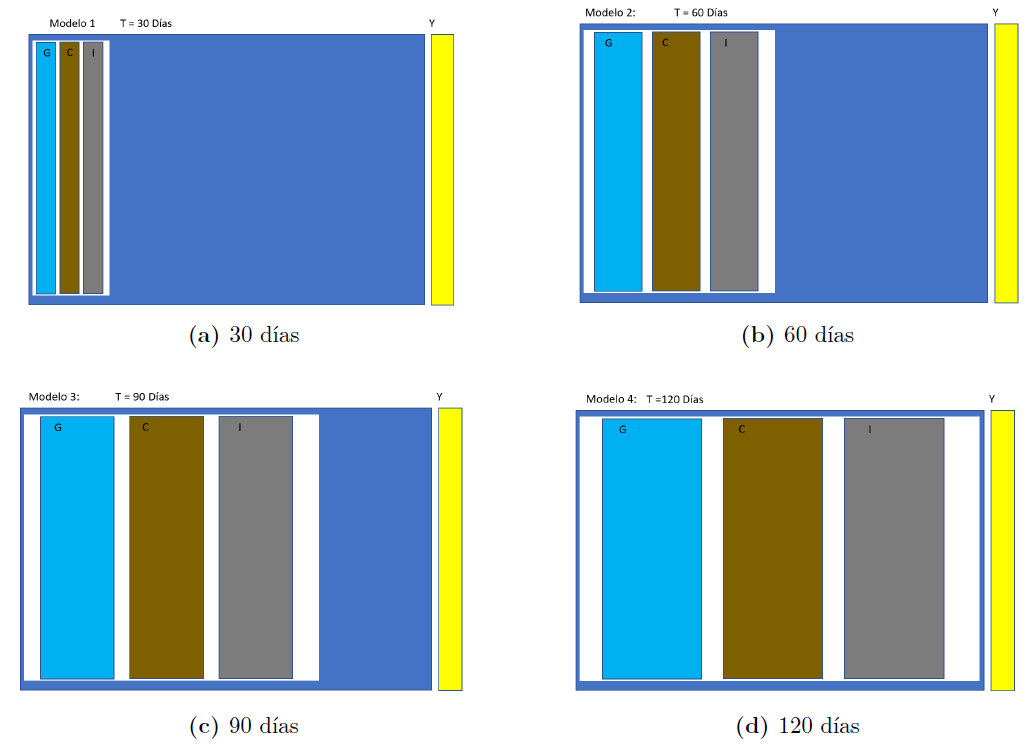
\includegraphics[width=0.7\linewidth]{figs/fig1}
		\caption{Figura 1.2. Rangos de tiempo utilizados en la predicción del abandono}
		\label{fig:fig1}
	\end{figure}
\end{frame}


%========= Diapositiva con ítems resaltados con colores:
\begin{frame}
	\frametitle{Subdivisión en bloques}
	La subdivisión en bloques permite un análisis más detallado de la red social en segmentos específicos de tiempo \citep{kim2012a}. Se consideraron diferentes rangos temporales y se determinaron las opciones de subdivisión en bloques. 
	\begin{table}[H]
		\centering
		\begin{tabular}{ll}
			\toprule
			Rangos & Número de días $\times$ Número de bloques \\
			\midrule
			30 días & 5 $\times$ 6, 10 $\times$ 3, 15 $\times$ 2 \\
			60 días & 5 $\times$ 12, 10 $\times$ 6, 15 $\times$ 4, 20 $\times$ 3, 30 $\times$ 2 \\
			90 días & 5 $\times$ 18, 10 $\times$ 9, 15 $\times$ 6, 30 $\times$ 3, 45 $\times$ 2 \\
			120 días & 5 $\times$ 24, 10 $\times$ 12, 15 $\times$ 8, 20 $\times$ 6, 30 $\times$ 4, 40 $\times$ 3, 60 $\times$ 2 \\
			\bottomrule
		\end{tabular}
		\caption{Tabla 1.2. Subdivisión en bloques para cada rango temporal.}
		
		\label{tab:subdivision-bloques1}
	\end{table}

\end{frame}


%========= Diapositiva con ítems resaltados con colores:
\begin{frame}
	\frametitle{Subdivisión en bloques seriados secuencialmente}
	\begin{figure}
		\centering
		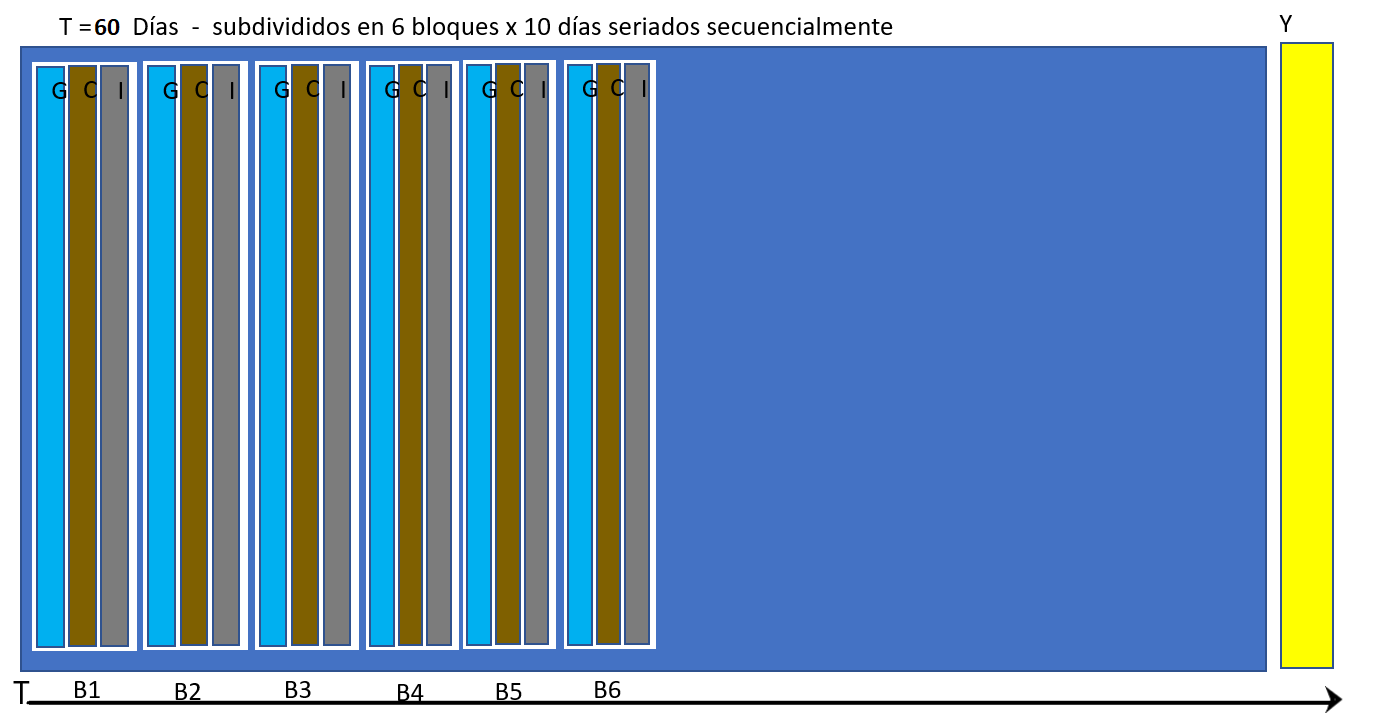
\includegraphics[width=0.7\linewidth]{figs/imagen20t}
		\caption{Figura 1.3. Subdivisión del rango de tiempo en bloques seriados secuencialmente}
		\label{fig:imagen320}
	\end{figure}
	
\end{frame}


%========= Diapositiva con ítems resaltados con colores:
\begin{frame}
	\frametitle{Subdivisión en bloques dinámicos o encadenados}
	\begin{itemize}
		\item La subdivisión en \textbf{bloques secuenciales} permite analizar las interacciones y dinámicas dentro de cada bloque. La subdivisión en bloques dinámicos o encadenados establece una relación de continuidad entre los bloques, capturando la evolución y los cambios a largo plazo \citep{Mahmoud_2021,  tang2010a}.
		\item En la subdivisión en \textbf{bloques encadenados}, cada bloque temporal se superpone con el bloque anterior y el bloque siguiente. 
		\item Esto significa que se comparten nodos y conexiones entre bloques adyacentes, lo que permite capturar la continuidad y los cambios graduales en la red a lo largo del tiempo.
	\end{itemize}	
\end{frame}

%========= Diapositiva con ítems resaltados con colores:
\begin{frame}
	\frametitle{Subdivisión en bloques dinámicos o encadenados}
	\begin{figure}[H]
		\centering
		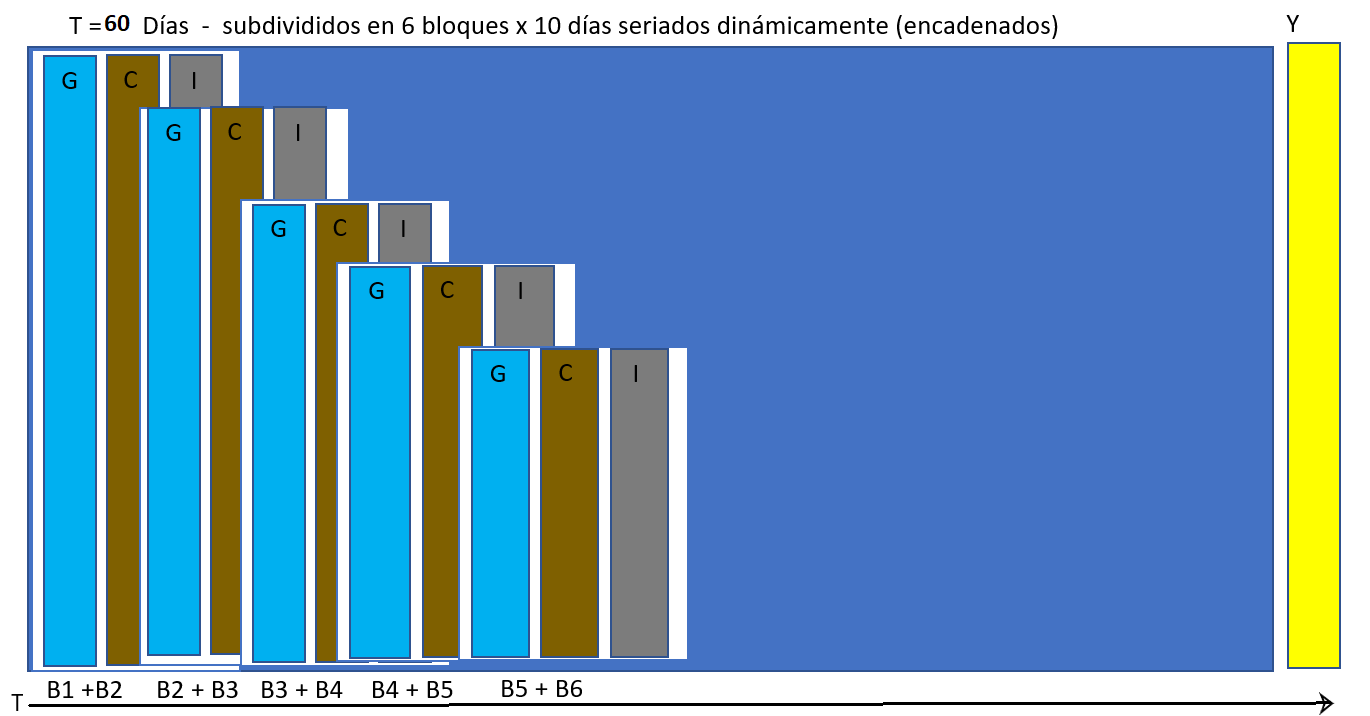
\includegraphics[width=0.7\linewidth]{figs/imagen21t}
		\caption{Figura 1.4. Subdivisión del rango de tiempo en bloques seriados dinámicamente (encadenados)}
	\end{figure}
	
\end{frame}



\subsection{Subobjetivos e hipótesis}
%========= Diapositiva con ítems resaltados con colores:
\begin{frame}
	\frametitle{Subbjetivos e hipótesis: Teorías del Aprendizaje Social}
	\begin{block}{Subobjetivo 1: Teoría del capital social de la red}
		\textbf{Hipótesis A}: Las medidas de centralidad ponderadas serán más capaces de capturar la importancia de las interacciones entre los nodos y predecir el abandono estudiantil \citep{wasko_why_2005, barrat2004a}.
		
	\end{block}
	\begin{block}{Subobjetivo 2: Teoría de la estructura social de la red}
		\textbf{Hipótesis B}: Los modelos de medidas de centralidad globales serán más eficaces para predecir el abandono estudiantil en comparación con los modelos que solo consideran medidas locales \citep{krause_social_2007, abbasi2013a, Mahmoud_2021}.
		
	\end{block}
	\begin{block}{Subobjetivo 3: Teoría del balance social de la red}
		\textbf{Hipótesis C}: Las medidas de centralidad junto a las medidas de sentimiento expresadas en los mensajes podrán predecir el abandono estudiantil de manera más precisa \citep{kim2012a, rawlings_structural_2017, marcos_learning_2019}.
	\end{block}
\end{frame}

\subsection{Atributos}

\begin{frame}
	\frametitle{Medidas de Centralidad en Redes Sociales}

\begin{block}{Medidas de Centralidad}
	\begin{enumerate}
	\item \textbf{Grado (Degree)}: número de enlaces que tiene un nodo. 
	
	\item \textbf{Cercanía (Closeness)}: distancia promedio a los demás nodos. 
	
	\item \textbf{Intermediación (Betweenness)}: cuántas veces un nodo se encuentra en el camino más cortos entre otros nodos.
	\end{enumerate}
\end{block}

\begin{block}{Medidas de Centralidad Ponderadas}
	\begin{enumerate}
		\item \textbf{Sin pesos}: consideran solo la cantidad de nodos vecinos.
		\item \textbf{Con pesos}: incluye la frecuencia de interacción con los nodos vecinos.
	\end{enumerate}
\end{block}

\begin{block}{Medidas de Centralidad Locales y Globales}
	\begin{enumerate}
		\item \textbf{Local}: mide la relación del nodo con sus vecinos directos.
		\item \textbf{Global o híbridas}: mide las interacciones de los nodos vecinos a los que un nodo está conectado.
	\end{enumerate}
\end{block}

	
\end{frame}




\begin{frame}
	\frametitle{Medidas de Sentimiento y Emoción}
	\begin{block}{Sentimiento}
		\begin{itemize}
			\item Métrica utilizada para evaluar el \textbf{tono emocional} transmitido en los mensajes de texto. Asigna un valor numérico entre 0 y 1 representando la probabilidad de que el texto sea "positivo".
		\end{itemize}
	\end{block}
	
	\begin{block}{Russel Valence y Russel Arousal}
		\begin{itemize}
			\item \textbf{Russel Valence}: Métrica que evalúa la carga emocional o la valencia de un texto.
			\item \textbf{Russel Arousal}: Métrica que evalúa el nivel de excitación o activación emocional transmitido por un texto.
		\end{itemize}
	\end{block}
	
	\begin{block}{Emoción}
		\begin{itemize}
			\item Utiliza una \textbf{región de Russel} para clasificar el texto en categorías emocionales como neutro, relajado, feliz, triste o enfadado.
		\end{itemize}
	\end{block}
	
\end{frame}




\section{Procesamiento de datos y técnicas  de aprendizaje supervisado}
%========= Diapositiva con ítems resaltados con colores:
\begin{frame}
	\frametitle{Algoritmos de aprendizaje y métricas de rendimiento}
	
\begin{columns}[t]
	\column{0.5\textwidth}
	\textbf{Algoritmos de aprendizaje supervisado:}
	\begin{itemize}
		\item \textcolor{blue}{Regresión Logística}
		\item \textcolor{blue}{SVM (Support Vector Machine)}
		\item \textcolor{blue}{Decision Tree Classifier}
		\item \textcolor{blue}{KNN (K-Nearest Neighbors)}
		\item \textcolor{blue}{MLP Classifier (Multi-Layer Perceptron)}
	\end{itemize}
	
	\column{0.5\textwidth}
	\textbf{Métricas de evaluación de la predicción:}
	\begin{itemize}
		\item \textcolor{red}{Precisión (Accuracy)}
		\item \textcolor{red}{Precisión (Precision)}
		\item \textcolor{red}{Exhaustividad (Recall)}
		\item \textcolor{red}{Puntuación F1 (F1 Score)}
		\item \textcolor{red}{ROC AUC (Area Under the ROC Curve)}
	\end{itemize}
	
\end{columns}
	
\end{frame}
%
%%========= Diapositiva con ítems resaltados con colores:
%\begin{frame}
%	\frametitle{Algoritmos de aprendizaje supervisado}
%	
%	\begin{itemize}
%		\item Regresión Logística: Clasificación binaria basada en un modelo logístico.
%		\item SVM (Support Vector Machine): Clasificación y regresión basada en hiperplanos óptimos en un espacio de alta dimensionalidad.
%		\item Decision Tree Classifier: Toma de decisiones basada en una estructura de árbol que divide los datos según características.
%		\item KNN (K-Nearest Neighbors): Clasificación basada en los K puntos de entrenamiento más cercanos en función de la distancia.
%		\item MLP Classifier (Multi-Layer Perceptron): Clasificación basada en redes neuronales artificiales con múltiples capas de nodos.
%	\end{itemize}
%	
%\end{frame}
%
%
%\begin{frame}
%	\frametitle{Métricas de evaluación de la predicción}
%	\begin{itemize}
%		\item Precisión (Accuracy): Proporción de predicciones correctas sobre el total de predicciones realizadas.
%		\item Precisión (Precision): Proporción de verdaderos positivos sobre el total de positivos predichos. Indica qué tan bien el modelo identifica correctamente los casos positivos.
%		\item Exhaustividad (Recall): Proporción de verdaderos positivos sobre el total de positivos reales. Indica qué tan bien el modelo captura todos los casos positivos.
%		\item Puntuación F1 (F1 Score): Media armónica de la precisión y la exhaustividad. Proporciona una medida equilibrada del rendimiento del modelo.
%		\item ROC AUC (Area Under the Receiver Operating Characteristic Curve): Capacidad de discriminación del modelo y su habilidad para distinguir entre las clases positiva y negativa.
%	\end{itemize}
%	
%\end{frame}



%========= Diapositiva con ítems resaltados con colores:

\begin{frame}
	\frametitle{Índices de evaluación de las redes sociales dinámicas en la predicción}
	\begin{block}{Evaluamos las teorías e hipótesis propuestas utilizando índices construidos específicos.}
	\begin{itemize}
		\item \textbf{Índice de amplitud o cobertura de la información}: mide la proporción del tiempo total de la asignatura cubierta por cada rango de tiempo analizado en los foros de los estudiantes.
		%Mide la capacidad del algoritmo para capturar la diversidad de interacciones en la red social dinámica.
		\item \textbf{Índice de unidad de información}: evalúa el grado de subdivisión en bloques que se utiliza para obtener las medidas de posición de los estudiantes y de expresión de sentimientos.
		%Evalúa la capacidad del algoritmo para identificar grupos o comunidades dentro de la red social dinámica.
		\item \textbf{Índice de cantidad de información}: es una medida que combina el grado de subdivisión en bloques y la proporción de cobertura temporal en el análisis de redes sociales.
		%Cuantifica la cantidad de información relevante proporcionada por el algoritmo sobre las interacciones en la red social dinámica.
	\end{itemize}
	\end{block}
\end{frame}



\section{Resultados Clave}

%========= Diapositiva con ítems resaltados con colores:
\begin{frame}
	\frametitle{Resumen teorías, hipótesis e índices}
	
	\begin{figure}[H]
		\centering
		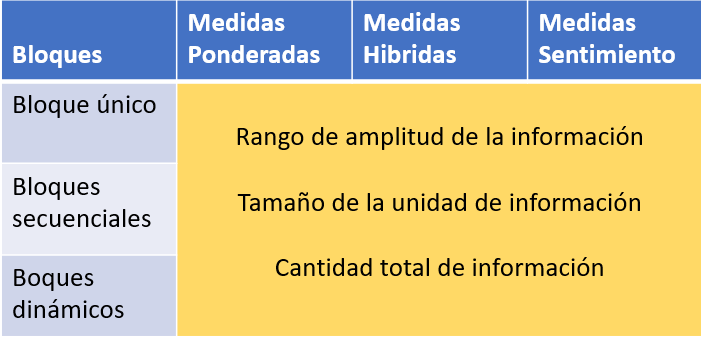
\includegraphics[width=0.9\linewidth]{figs/imagen23}
		\caption{Figura 1.5. Resumen de teorías, hipótesis e índices}
		\label{fig:imagen23}
	\end{figure}
\end{frame}

\begin{frame}
	\frametitle{Modelos predictivos por combinación de factores}
	
	\begin{figure}[H]
		\centering
		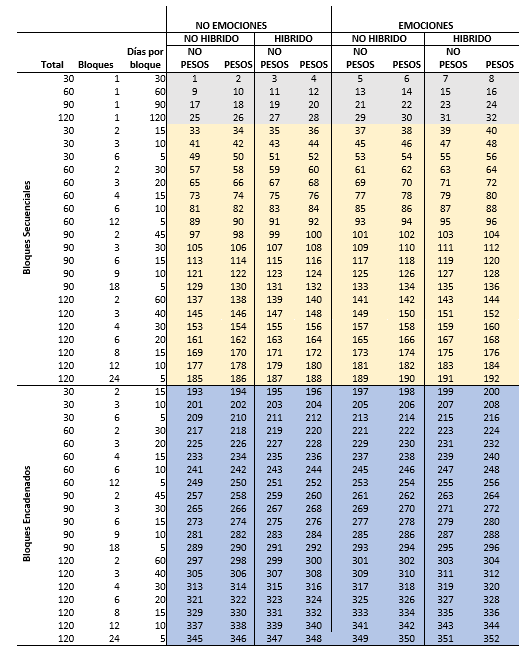
\includegraphics[width=0.5\linewidth]{figs/imagen32}
		\caption{Figura 1.6. Modelos predictivos por combinación de factores.}
		\label{fig:imagen32}
	\end{figure}
\end{frame}


\subsection{ Objetivo 1 - Rangos Temporales}


%%========= Diapositiva con ítems resaltados con colores:
\begin{frame}
	\frametitle{Objetivo 1: Analizar la eficacia de las predicciones utilizando distintos rangos de tiempo}
	\begin{block}{Rangos de tiempo (todos los tipos de subdivisión temporal).} 
		Con un rango de \textcolor{blue}{60} o \textcolor{blue}{90} días se obtienen predicciones precisas del abandono.
		
	\end{block}
	\begin{columns}[c]
		% create the column with the first image, that occupies
		% half of the slide
		\begin{column}{.5\textwidth}
			\begin{figure}
				\centering
				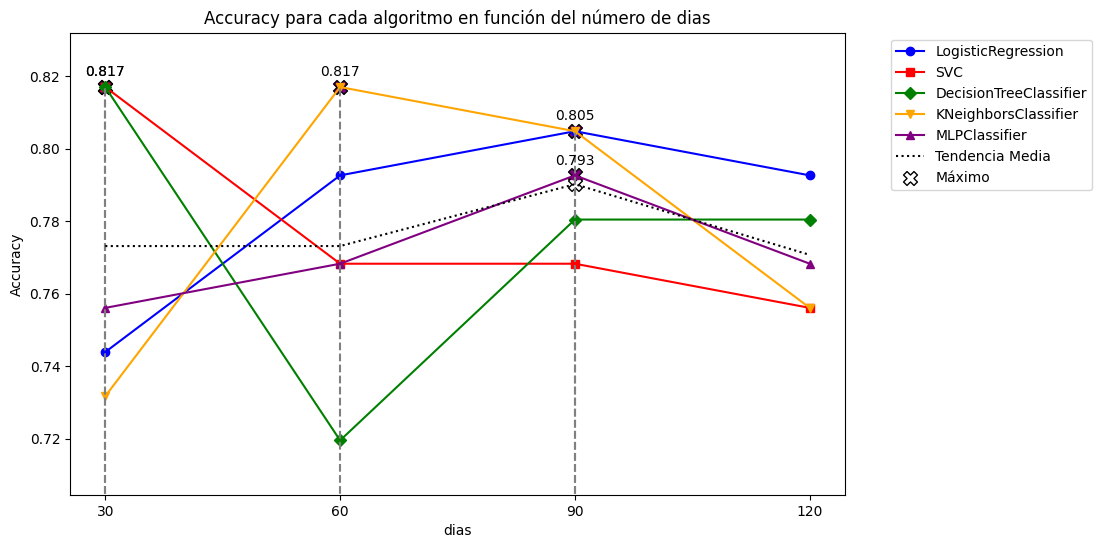
\includegraphics[width=1\textwidth]{figs/cap6/figura_1}
				\caption{Figura 7.1. Máximo Accuracy por rango temporal}
			\end{figure}      
		\end{column}
		% create the column with the second image, that also
		% occupies half of the slide
		\begin{column}{.5\textwidth}
			\begin{figure}
				\centering
				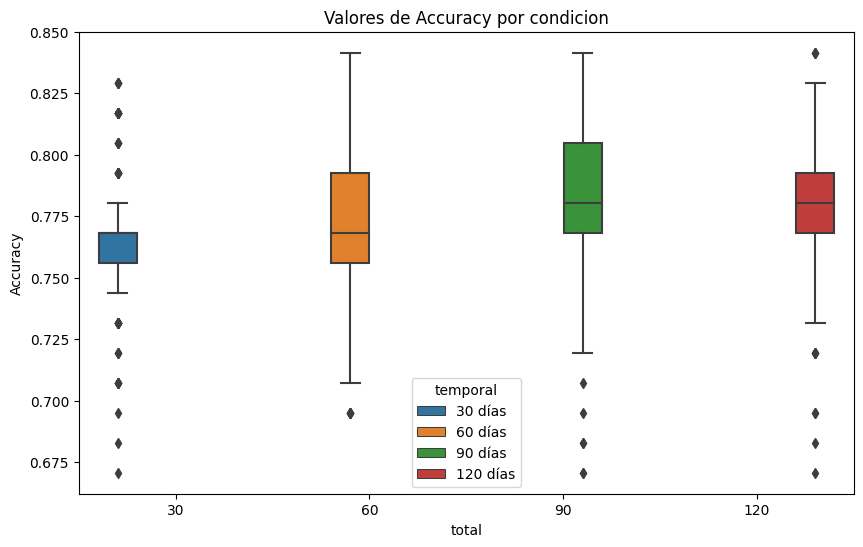
\includegraphics[width=0.8\textwidth]{figs/cap7/figura_1}
				\caption{Figura 9.1. Distribución de Accuracy por rango temporal}
			\end{figure}
		\end{column}
	\end{columns}
	
\end{frame}
%%========= Diapositiva con ítems resaltados con colores:
\begin{frame}
	\frametitle{Objetivo 1: Analizar la eficacia de las predicciones utilizando distintos rangos de tiempo}
		\begin{block}{Rangos de tiempo (todos los tipos de subdivisión temporal).} 
	A medida que aumenta el porcentaje de \textcolor{blue}{cobertura temporal}, la \textcolor{red}{eficacia} de todos los tipos de algoritmos también \textcolor{blue}{incrementa}.

	\end{block}
	\begin{columns}[c]
		% create the column with the first image, that occupies
		% half of the slide
		\begin{column}{.5\textwidth}
			\begin{figure}
				\centering
				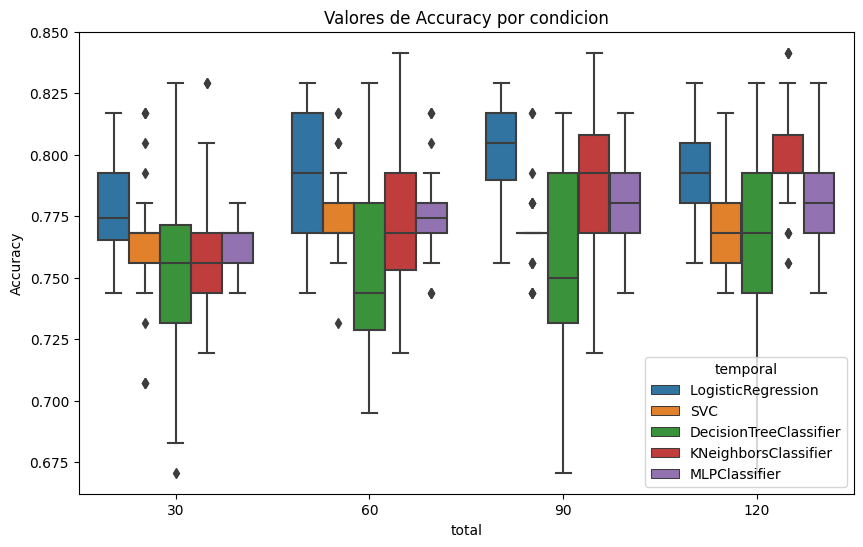
\includegraphics[width=0.8\textwidth]{figs/cap7/figura_19}
				\caption{Figura 9.3. Eficacia de los algoritmos por rangos temporales}
			\end{figure}      
		\end{column}
		% create the column with the second image, that also
		% occupies half of the slide
		\begin{column}{.5\textwidth}
			\begin{figure}
				\centering
				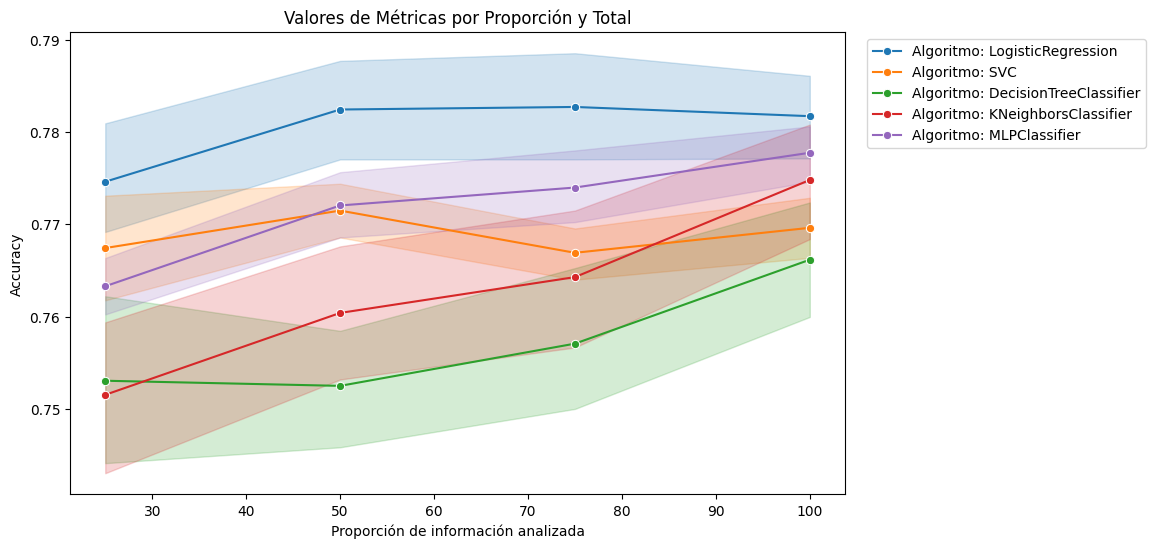
\includegraphics[width=1\textwidth]{figs/cap7/figura_14}
				\caption{Figura 9.5. Índice de amplitud de la información}
			\end{figure}
		\end{column}
	\end{columns}

\end{frame}

%%========= Diapositiva con ítems resaltados con colores:
\begin{frame}
	\frametitle{Objetivo 1: Analizar la eficacia de las predicciones utilizando distintos rangos de tiempo}
\begin{block}{Rangos de tiempo (todos los tipos de subdivisión temporal).} 
	El \textcolor{red}{punto óptimo} de eficacia en la predicción se encuentra con valores \textcolor{blue}{previos al máximo nivel de unidad} y \textcolor{blue}{cantidad de información}.

	\end{block}
	\begin{columns}[c]
		% create the column with the first image, that occupies
		% half of the slide
		\begin{column}{.5\textwidth}
			\begin{figure}
				\centering
				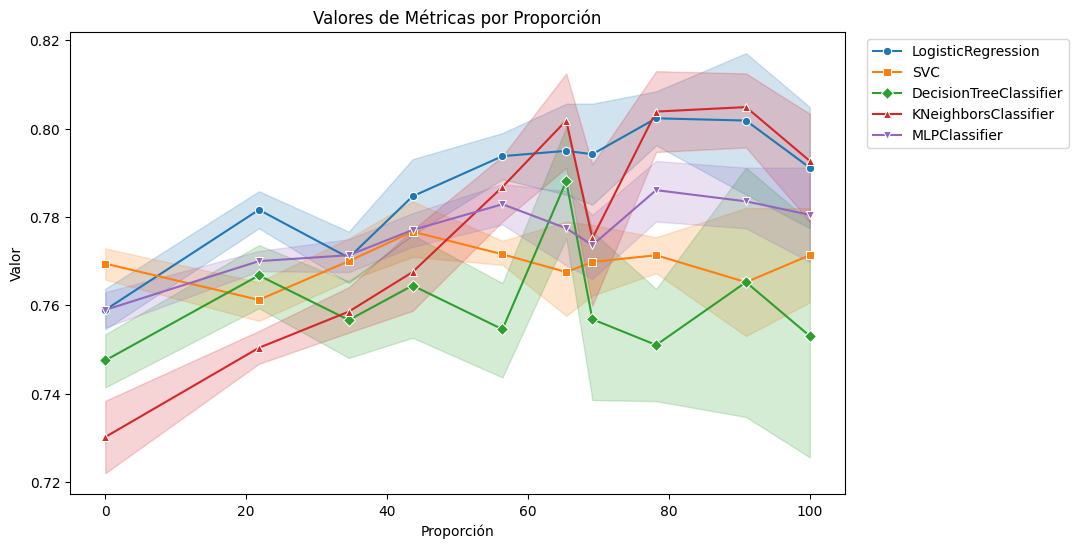
\includegraphics[width=1\textwidth]{figs/cap7/figura_12}
				\caption{Figura 9.6. Índice de unidad de información}
			\end{figure}      
		\end{column}
		% create the column with the second image, that also
		% occupies half of the slide
		\begin{column}{.5\textwidth}
			\begin{figure}
				\centering
				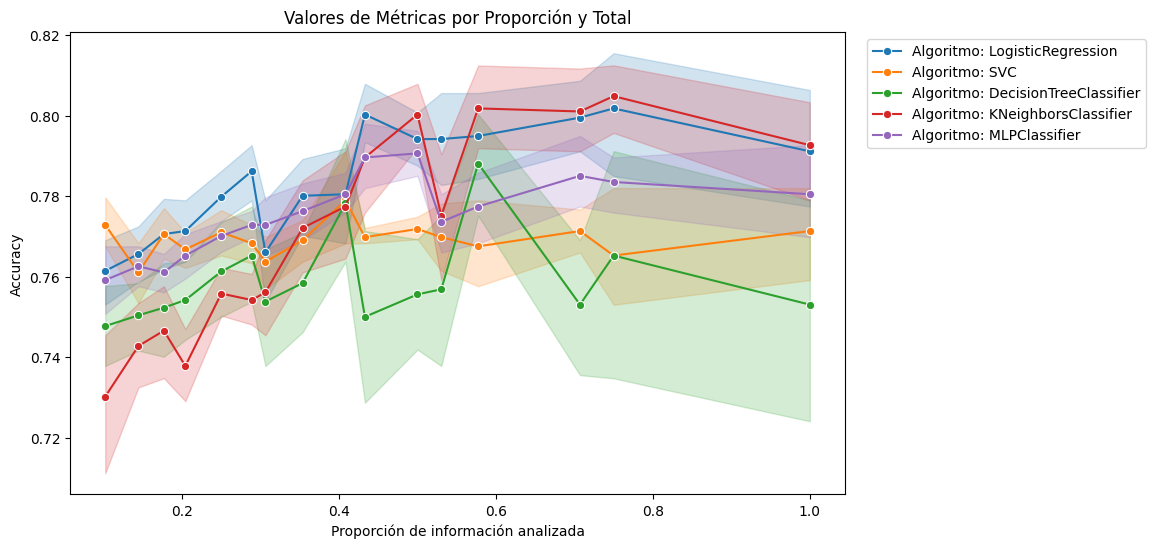
\includegraphics[width=1\textwidth]{figs/cap7/figura_13}
				\caption{Figura 9.7. Índice de cantidad de información}
			\end{figure}
		\end{column}
	\end{columns}

	
\end{frame}



%%%========= Diapositiva con ítems resaltados con colores:
%\begin{frame}
%	\frametitle{Resultados. Objetivo 1 - Rangos Temporales}
%	\begin{columns}[onlytextwidth,T]
%		\begin{column}{.5\textwidth}
%			\begin{figure}
%				\centering
%			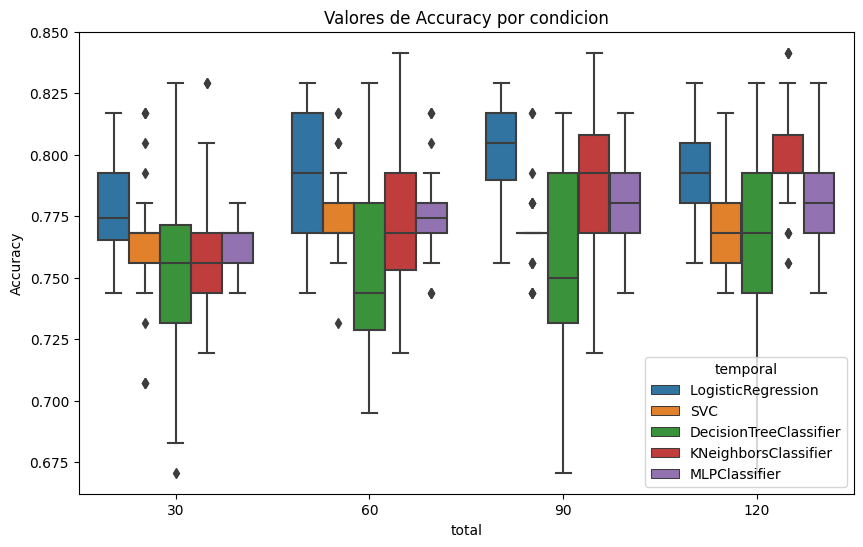
\includegraphics[width=0.5\textwidth]{figs/cap7/figura_19}
%			\caption{Precisión por rangos temporales}
%			\end{figure}      
%		\end{column}
%		\begin{column}{.5\textwidth}
%			\begin{figure}
%				\centering
%				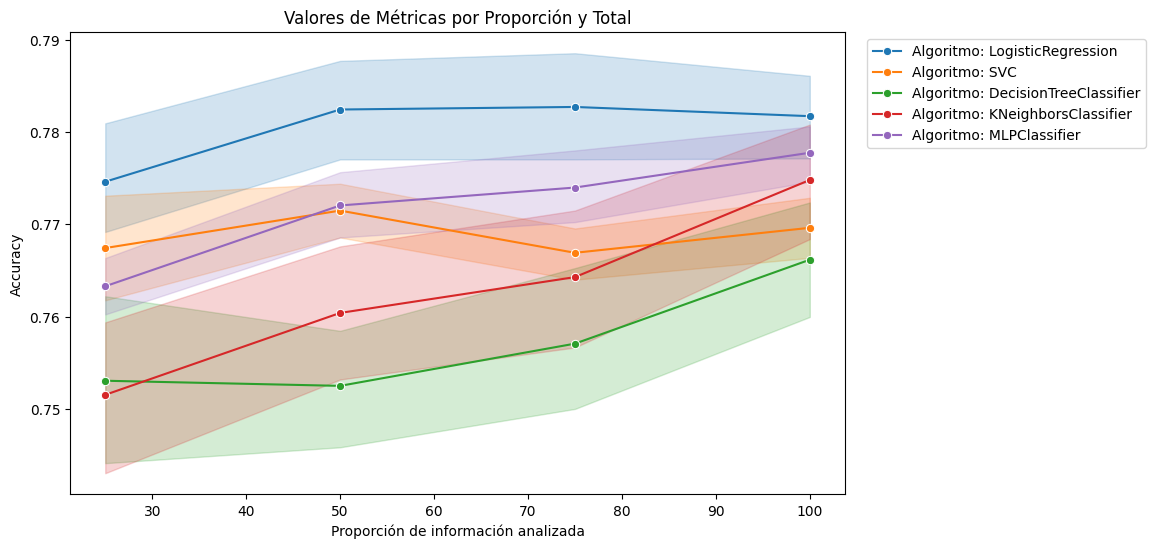
\includegraphics[width=0.6\textwidth]{figs/cap7/figura_14}
%
%			\caption{Índice de amplitud de información}
%			\end{figure}
%		\end{column}
%	\end{columns}
%	\begin{columns}[onlytextwidth,T]
%		\begin{column}{.5\textwidth}
%			\begin{figure}
%				\centering
%				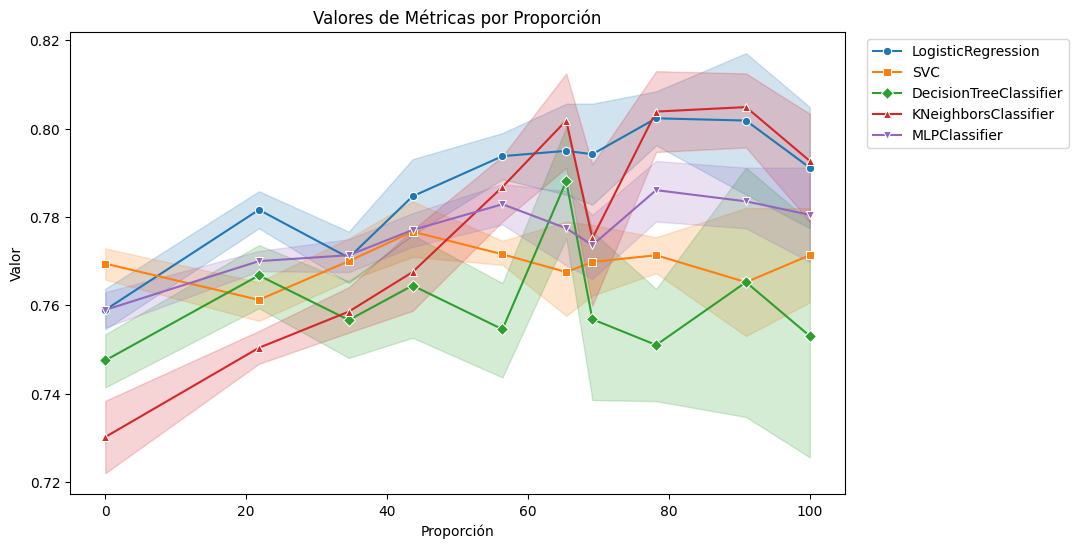
\includegraphics[width=0.6\textwidth]{figs/cap7/figura_12}
%			
%			\caption{Índice de unidad de información}
%			\end{figure}      
%		\end{column}
%		\begin{column}{.5\textwidth}
%			\begin{figure}
%				\centering
%				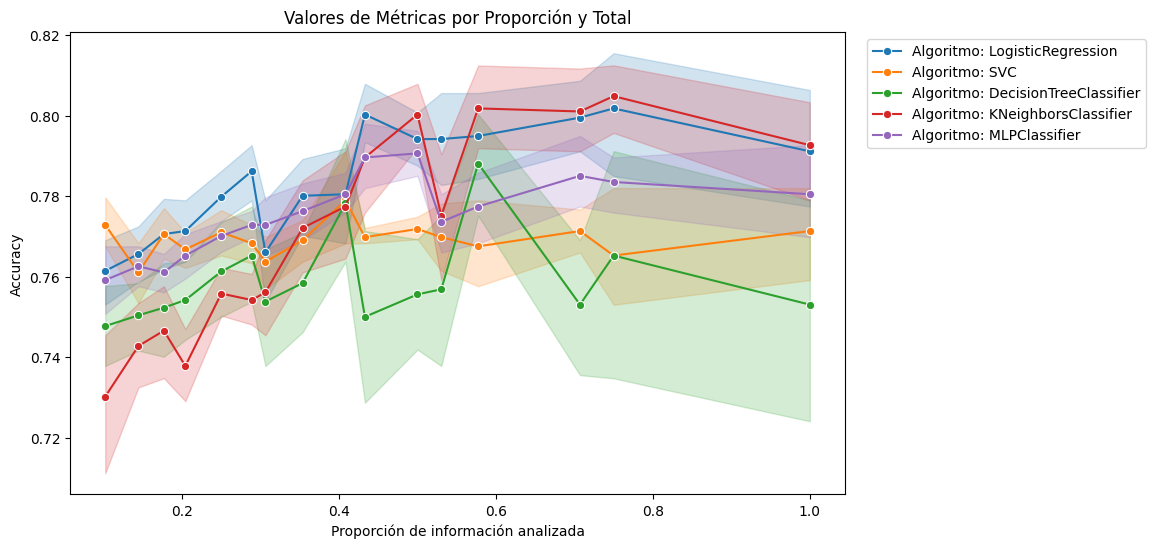
\includegraphics[width=0.6\textwidth]{figs/cap7/figura_13}
%				\caption{Índice de cantidad de información}
%			\end{figure}
%		\end{column}
%	\end{columns}
%\end{frame}



%
%%%========= Diapositiva con ítems resaltados con colores:
%\begin{frame}
%	\frametitle{Resultados. Objetivos 2 y 3: Tipo de bloques temporales}
%	\begin{columns}[onlytextwidth,T]
%		\begin{column}{.5\textwidth}
%			\begin{figure}
%				\centering
%				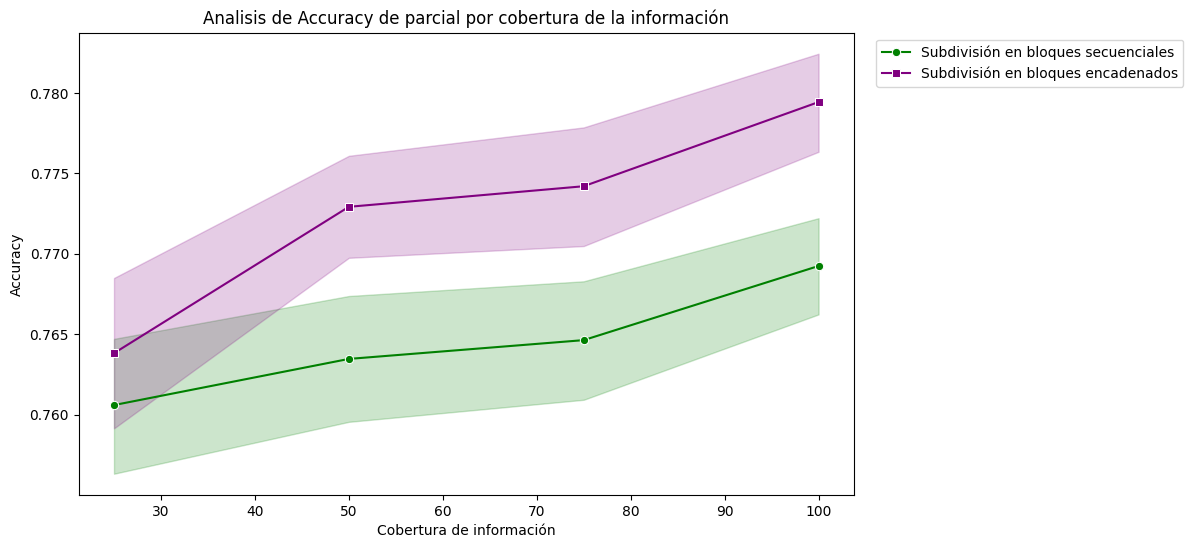
\includegraphics[width=0.5\textwidth]{figs/cap7/figura_15}
%				\caption{Índice de amplitud de información}
%			\end{figure}      
%		\end{column}
%		\begin{column}{.5\textwidth}
%			\begin{figure}
%				\centering
%				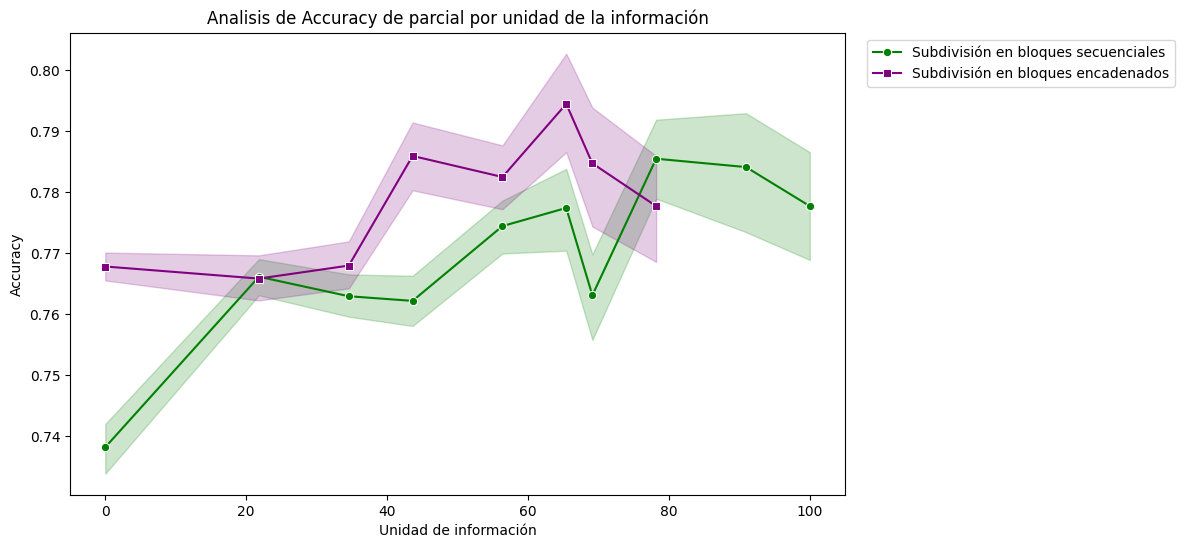
\includegraphics[width=0.6\textwidth]{figs/cap7/figura_16}
%				\caption{Índice de unidad de información}
%			\end{figure}
%		\end{column}
%	\end{columns}
%	\begin{columns}[onlytextwidth,T]
%		\begin{column}{.5\textwidth}
%			\begin{figure}
%				\centering
%				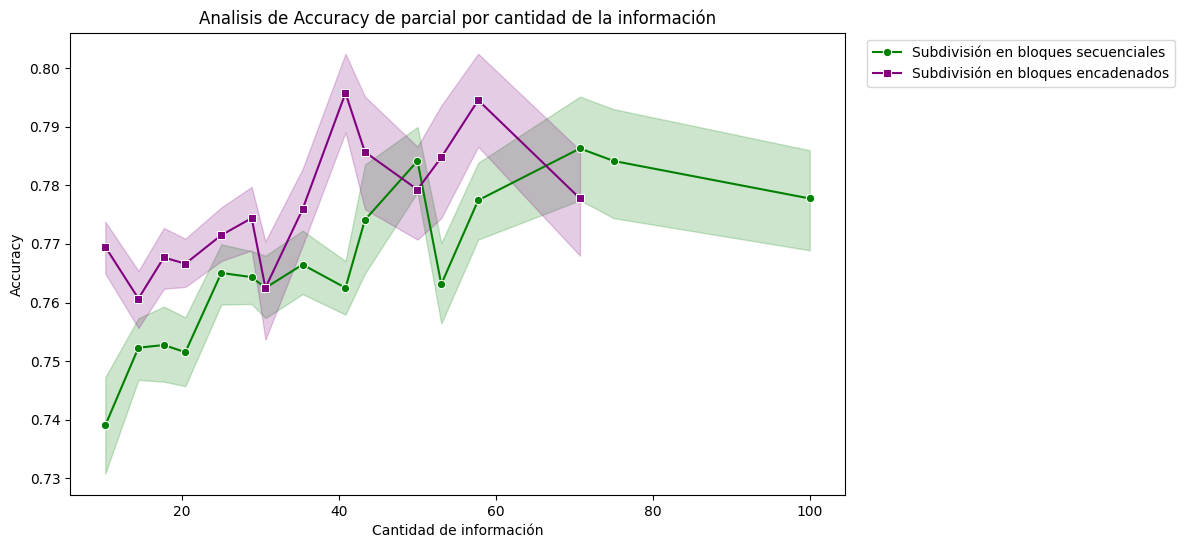
\includegraphics[width=0.6\textwidth]{figs/cap7/figura_17}
%				\caption{Índice de cantidad de información}
%			\end{figure}      
%		\end{column}
%		\begin{column}{.5\textwidth}
%			\begin{figure}
%				\centering
%				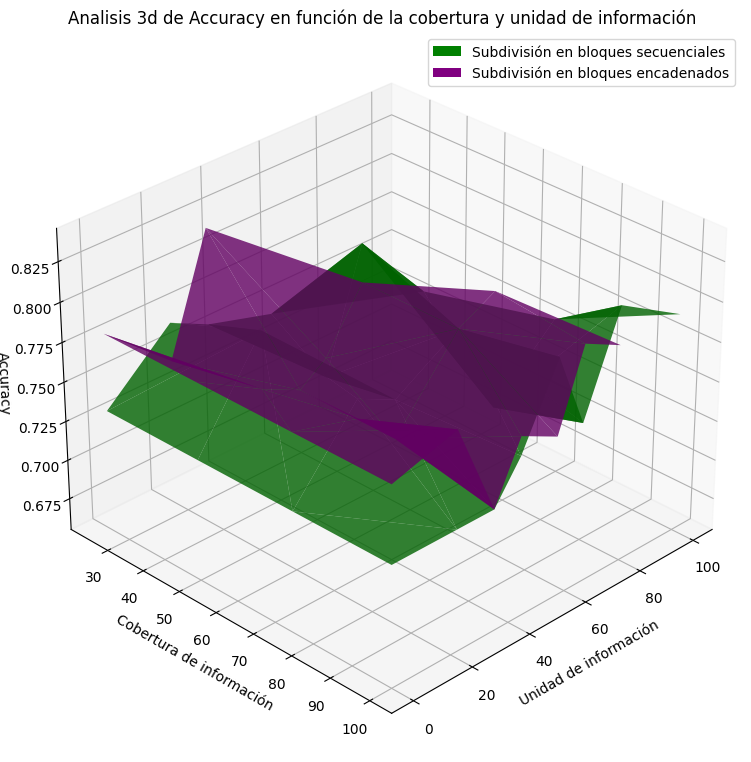
\includegraphics[width=0.6\textwidth]{figs/cap7/figura_18}
%			%	\caption{Índice de cantidad de información}
%			\end{figure}
%		\end{column}
%	\end{columns}
%\end{frame}


\subsection{ Objetivos 2 y 3: Tipo de bloques temporales}

%========= Diapositiva con ítems resaltados con colores:
\begin{frame}
	\frametitle{Objetivos 2 y 3: Analizar la eficacia de las predicciones utilizando distintos tipos de bloques temporales}
	\begin{block}{Tipos de subdivisión en bloques temporales: secuenciales vs encadenados.}
		La precisión de los algoritmos con bloques \textcolor{red}{encadenados} es ligeramente superior, especialmente en los rangos de tiempo intermedios de \textcolor{blue}{60} y \textcolor{blue}{90} días.
	\end{block}
	
	
	\begin{columns}[c]
		% create the column with the first image, that occupies
		% half of the slide
		\begin{column}{.5\textwidth}
			\begin{figure}
				\centering
				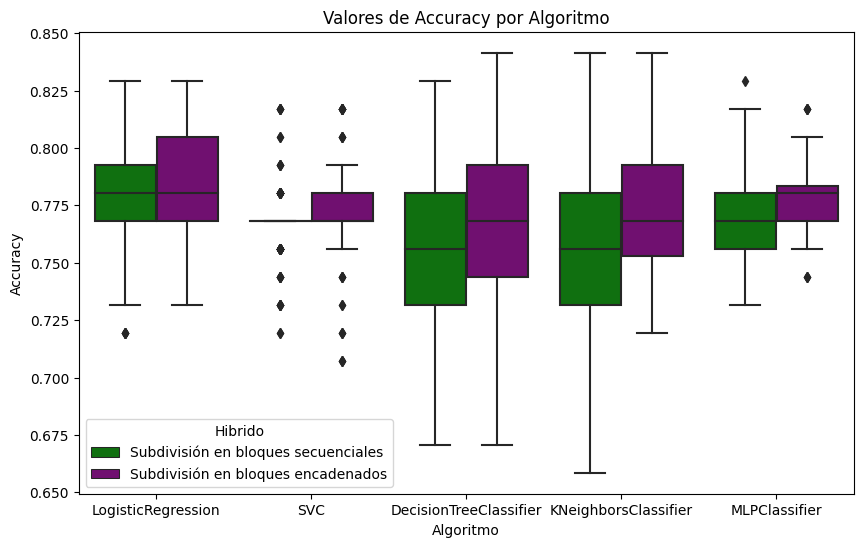
\includegraphics[width=0.9\textwidth]{figs/cap7/figura_24}
				\caption{Figura 9.10. Eficacia de los algoritmos por tipos de bloques}
			\end{figure}      
		\end{column}
		% create the column with the second image, that also
		% occupies half of the slide
		\begin{column}{.5\textwidth}
			\begin{figure}
				\centering
				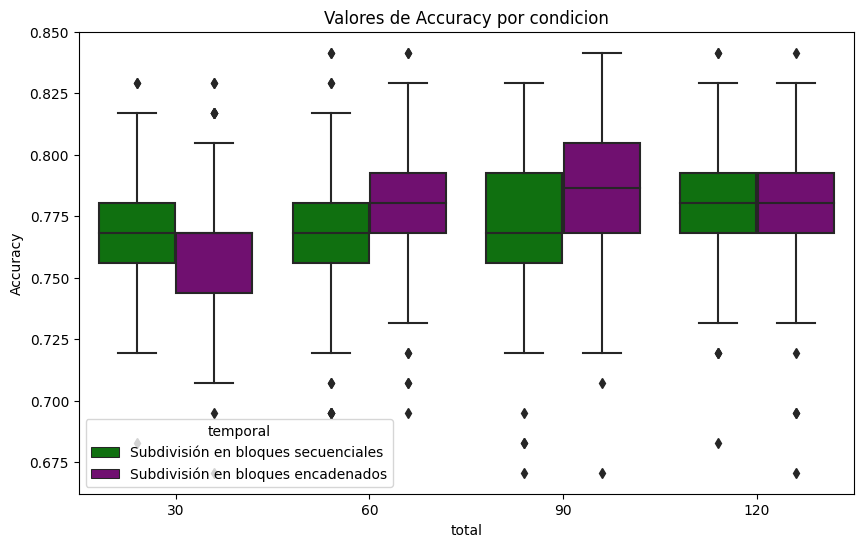
\includegraphics[width=0.9\textwidth]{figs/cap7/figura_6}
				\caption{Figura 9.8. Eficacia por rangos de tiempo y tipos de bloques.}
			\end{figure}
		\end{column}
	\end{columns}
	
\end{frame}

%%========= Diapositiva con ítems resaltados con colores:
\begin{frame}
	\frametitle{Objetivos 2 y 3: Analizar la eficacia de las predicciones utilizando distintos tipos de bloques temporales}
	\begin{block}{Tipos de subdivisión en bloques temporales: secuenciales vs encadenados.}
	La subdivisión en bloques \textcolor{blue}{encadenados} muestra una \textcolor{red}{eficacia superior} en comparación con la subdivisión en bloques \textcolor{blue}{secuenciales}.

	\end{block}
	
	\begin{columns}[c]
	% create the column with the first image, that occupies
	% half of the slide
	\begin{column}{.5\textwidth}
		\begin{figure}
			\centering
			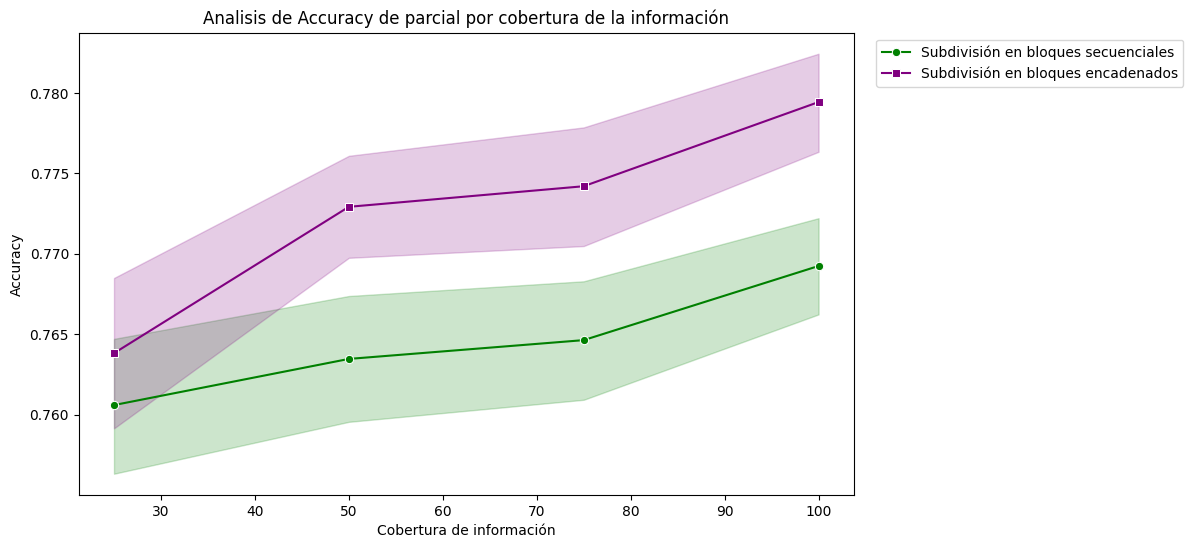
\includegraphics[width=1\textwidth]{figs/cap7/figura_15}
			\caption{Figura 9.12. Índice de amplitud de información}
		\end{figure}      
	\end{column}
	% create the column with the second image, that also
	% occupies half of the slide
	\begin{column}{.5\textwidth}
		\begin{figure}
			\centering
			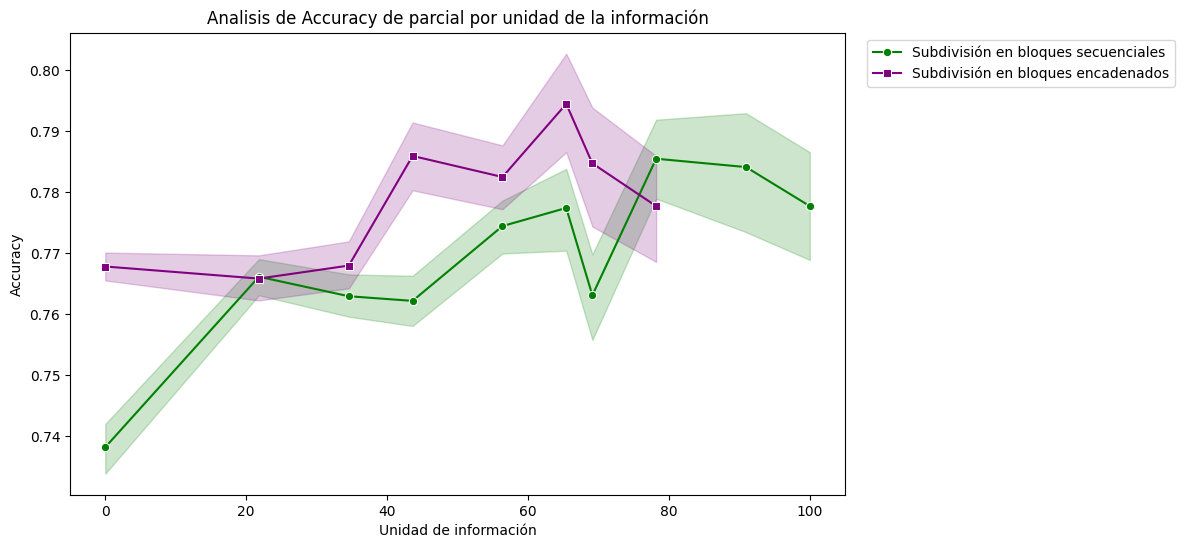
\includegraphics[width=1\textwidth]{figs/cap7/figura_16}
			\caption{Figura 9.13. Índice de unidad de información}
		\end{figure}
	\end{column}
\end{columns}

\end{frame}


%========= Diapositiva con ítems resaltados con colores:
\begin{frame}
	\frametitle{Objetivos 2 y 3: Analizar la eficacia de las predicciones utilizando distintos tipos de bloques temporales}
\begin{block}{Tipos de subdivisión en bloques temporales: secuenciales vs encadenados.}
	La subdivisión en bloques \textcolor{blue}{encadenados} aumenta la precisión (\textcolor{red}{Accuracy}) a medida que aumenta el \textcolor{blue}{rango de tiempo} y el tamaño de \textcolor{blue}{unidad} de la red.
	\end{block}
	

	\begin{columns}[c]
	% create the column with the first image, that occupies
	% half of the slide
	\begin{column}{.5\textwidth}
		\begin{figure}
			\centering
			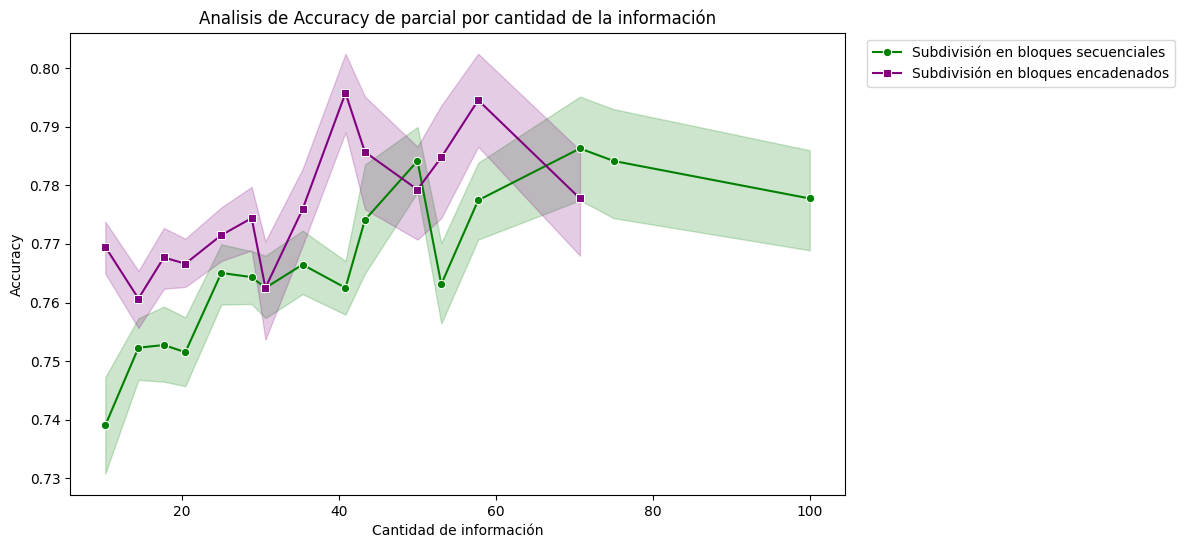
\includegraphics[width=1\textwidth]{figs/cap7/figura_17}
\caption{Figura 9.14. Índice de cantidad de información}
		\end{figure}      
	\end{column}
	% create the column with the second image, that also
	% occupies half of the slide
	\begin{column}{.5\textwidth}
		\begin{figure}
			\centering
			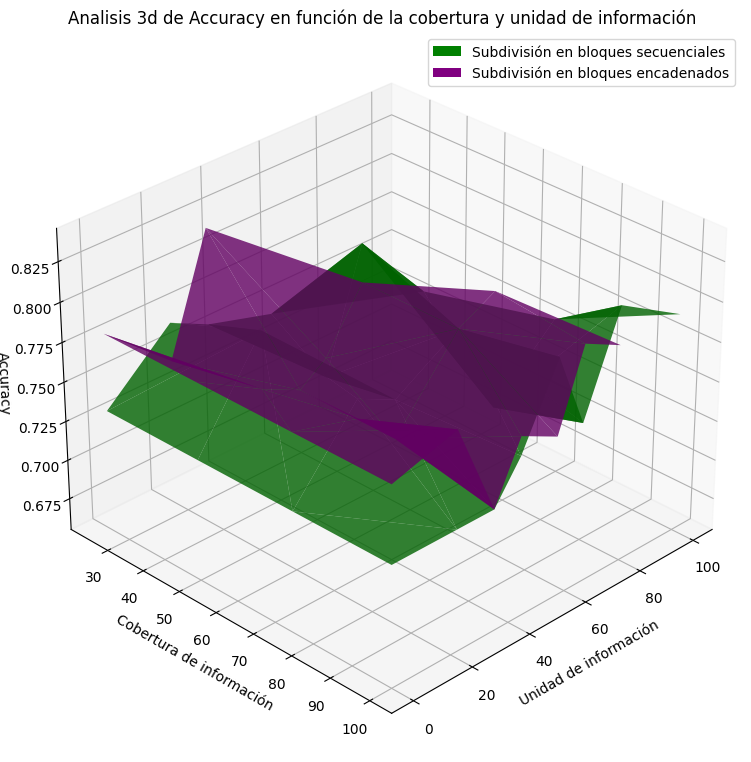
\includegraphics[width=0.6\textwidth]{figs/cap7/figura_18}
			\caption{Figura 9.15. Cobertura y unidad de información}
		\end{figure}
	\end{column}
\end{columns}
	
\end{frame}






\subsection{Subobjetivo 1: Hipótesis del Capital Social Cognitivo}


%========= Diapositiva con ítems resaltados con colores:
\begin{frame}
	\frametitle{Subobjetivo 1: Analizar la eficacia de las predicciones utilizando medidas centrales ponderadas (con pesos)}
	\begin{block}{Hipótesis del Capital Social Cognitivo}
		Las medidas de centralidad con \textcolor{blue}{pesos} tienden a ser igualmente efectivas para todos los algoritmos y ligeramente superiores en rangos de tiempo superiores al 50\% (\textcolor{red}{entre 60 y 120 días}).
	\end{block}
	\begin{columns}[c]
		% create the column with the first image, that occupies
		% half of the slide
		\begin{column}{.5\textwidth}
			\begin{figure}
				\centering
				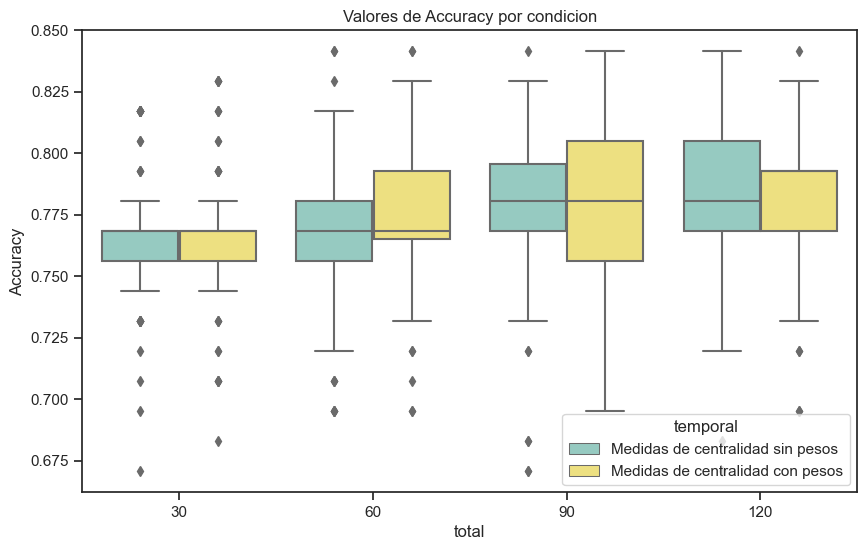
\includegraphics[width=0.8\textwidth]{figs/cap7/figura_29}
				\caption{Figura 10.1.  Eficacia por rangos de tiempo y tipos de medidas (ponderadas)}
			\end{figure}      
		\end{column}
		% create the column with the second image, that also
		% occupies half of the slide
		\begin{column}{.5\textwidth}
			\begin{figure}
				\centering
				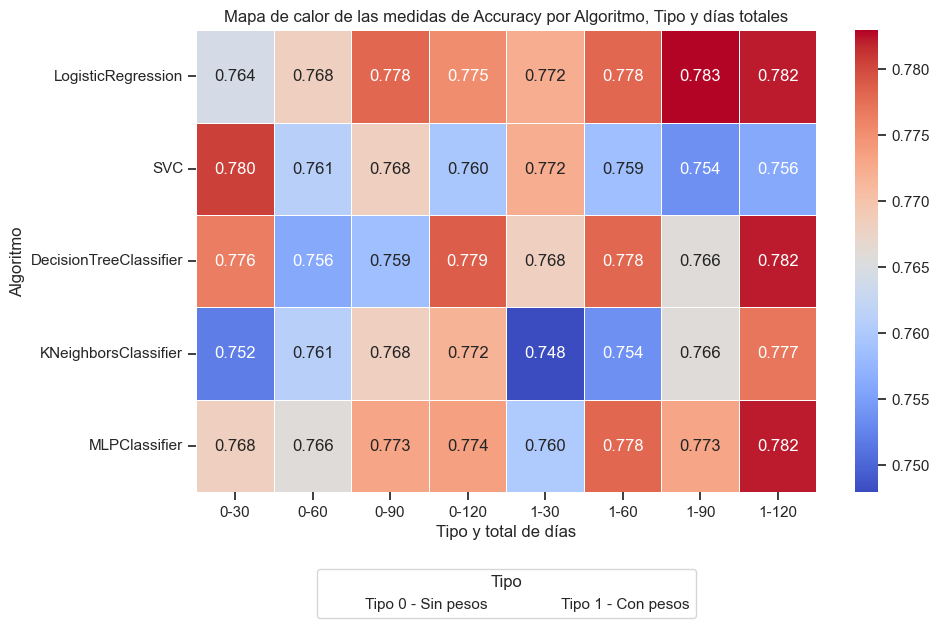
\includegraphics[width=0.8\textwidth]{figs/cap7/figura_73}
				\caption{Figura 7.65. Eficacia de los algoritmos por tipos de medidas (ponderadas)}
				
			\end{figure}
		\end{column}
	\end{columns}
	
\end{frame}


%%========= Diapositiva con ítems resaltados con colores:
\begin{frame}
	\frametitle{Subobjetivo 1: Analizar la eficacia de las predicciones utilizando medidas centrales ponderadas (con pesos)}
\begin{block}{Hipótesis del Capital Social Cognitivo}
No se observan diferencias entre medidas de centralidad \textcolor{blue}{sin pesos} y  \textcolor{red}{ponderadas} para predecir el abandono de la asignatura.
\end{block}

		\begin{columns}[c]
		% create the column with the first image, that occupies
		% half of the slide
		\begin{column}{.5\textwidth}
			\begin{figure}
				\centering
				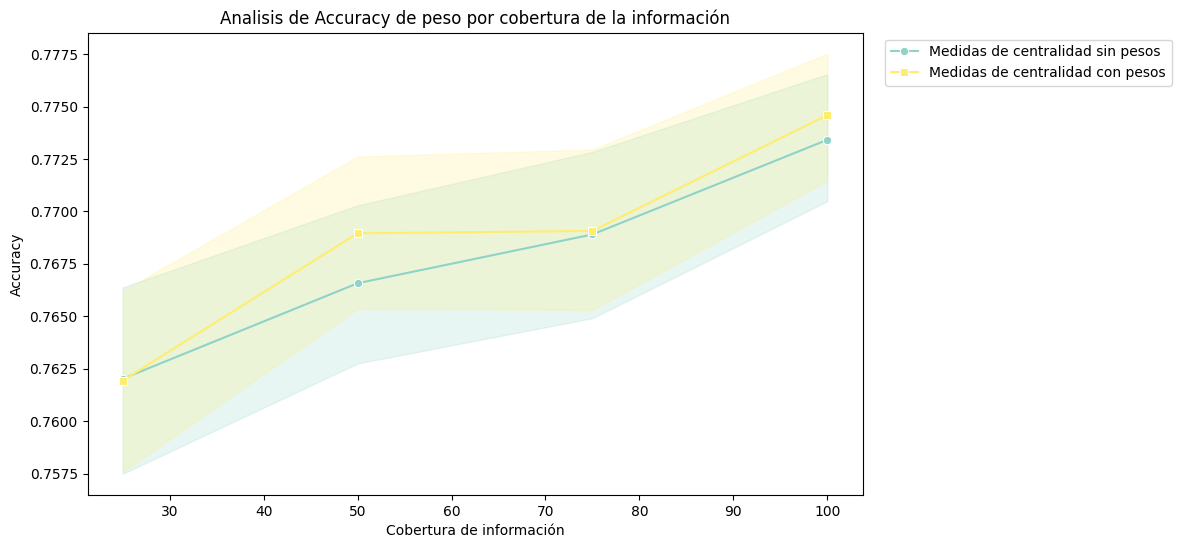
\includegraphics[width=1\textwidth]{figs/cap7/figura_34}
				\caption{Figura 10.3. Índice de amplitud de información}
			\end{figure}      
		\end{column}
		% create the column with the second image, that also
		% occupies half of the slide
		\begin{column}{.5\textwidth}
			\begin{figure}
				\centering
			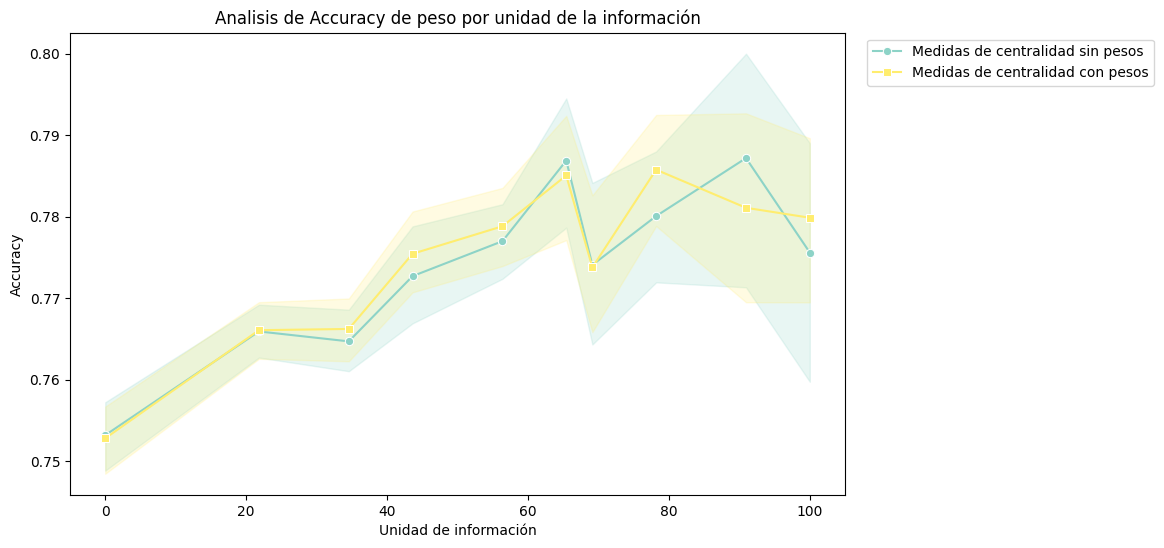
\includegraphics[width=1\textwidth]{figs/cap7/figura_35}
				\caption{Figura 10.4. Índice de unidad de información}
			\end{figure}
		\end{column}
		\end{columns}
			
\end{frame}


%========= Diapositiva con ítems resaltados con colores:
\begin{frame}
	\frametitle{Subobjetivo 1: Analizar la eficacia de las predicciones utilizando medidas centrales ponderadas (con pesos)}
\begin{block}{Hipótesis del Capital Social Cognitivo}
Las medidas de centralidad con \textcolor{blue}{pesos} tienden a ser más precisas cuando se dispone de una cantidad de información superior al \textcolor{red}{50\%}.
\end{block}
		\begin{columns}[c]
	% create the column with the first image, that occupies
	% half of the slide
	\begin{column}{.5\textwidth}
		\begin{figure}
			\centering
			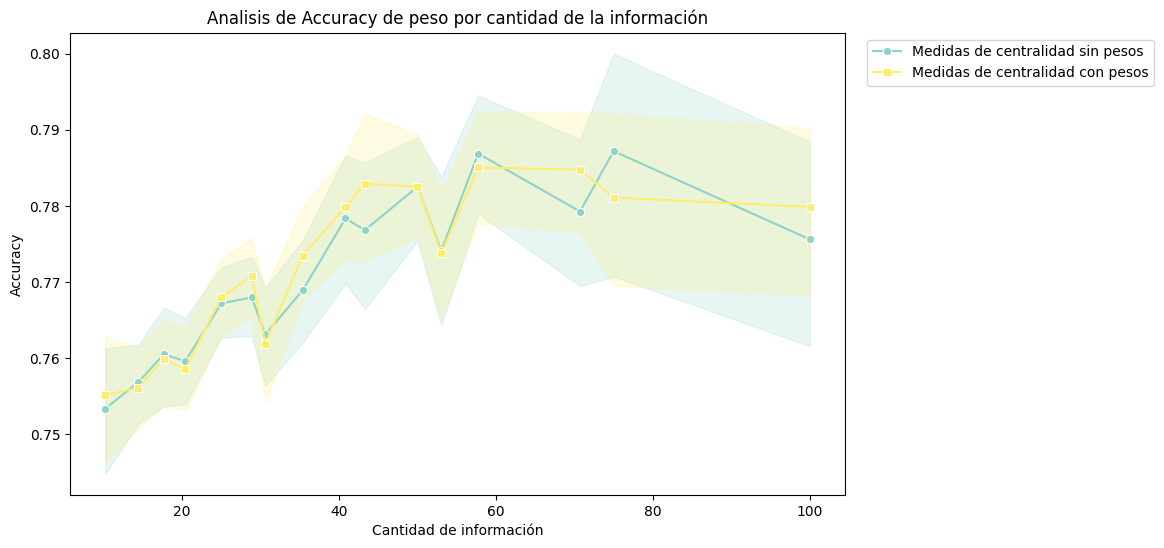
\includegraphics[width=1\textwidth]{figs/cap7/figura_36}
\caption{Figura 10.5. Índice de cantidad de información}
		\end{figure}      
	\end{column}
	% create the column with the second image, that also
	% occupies half of the slide
	\begin{column}{.5\textwidth}
		\begin{figure}
			\centering
			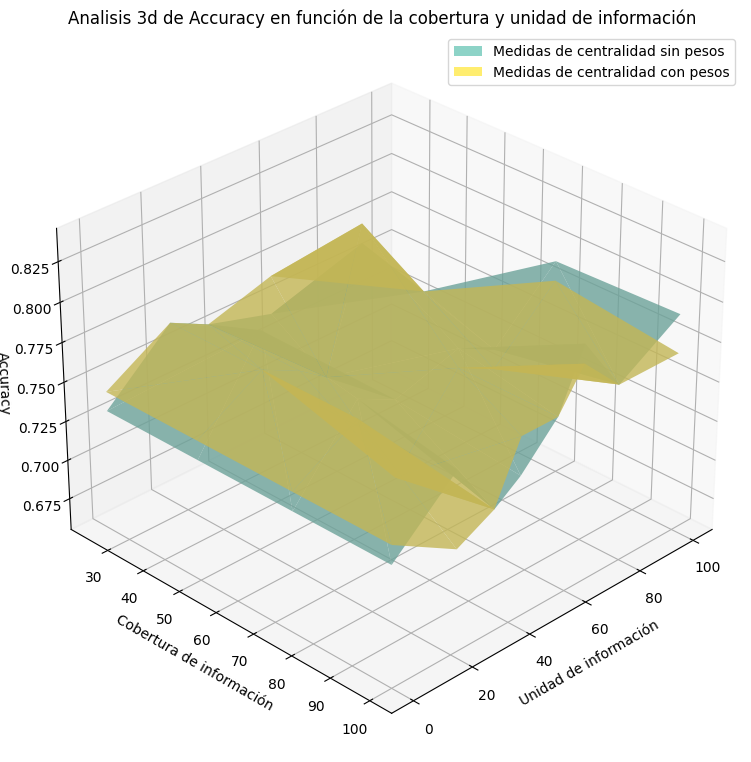
\includegraphics[width=0.6\textwidth]{figs/cap7/figura_37}
			\caption{Figura 10.6. Cobertura y unidad de información}
		\end{figure}
	\end{column}
\end{columns}
	
\end{frame}



\subsection{Subobjetivo 2: Hipótesis del Esquema Social Cognitivo}


%========= Diapositiva con ítems resaltados con colores:
\begin{frame}
	\frametitle{Subobjetivo 2: Analizar la eficacia de las predicciones utilizando medidas centrales  locales vs globales (híbridas)}
	\begin{block}{Hipótesis de la Estructura Social Cognitivo }
		Las medidas de centralidad \textcolor{blue}{globales} son igualmente precisas por tipo de algoritmos de aprendizaje supervisado, y ligeramente superiores a las \textcolor{blue}{locales} cuando el rango de tiempo es mayor.
	\end{block}
	\begin{columns}[c]
		% create the column with the first image, that occupies
		% half of the slide
		\begin{column}{.5\textwidth}
			\begin{figure}
				\centering
				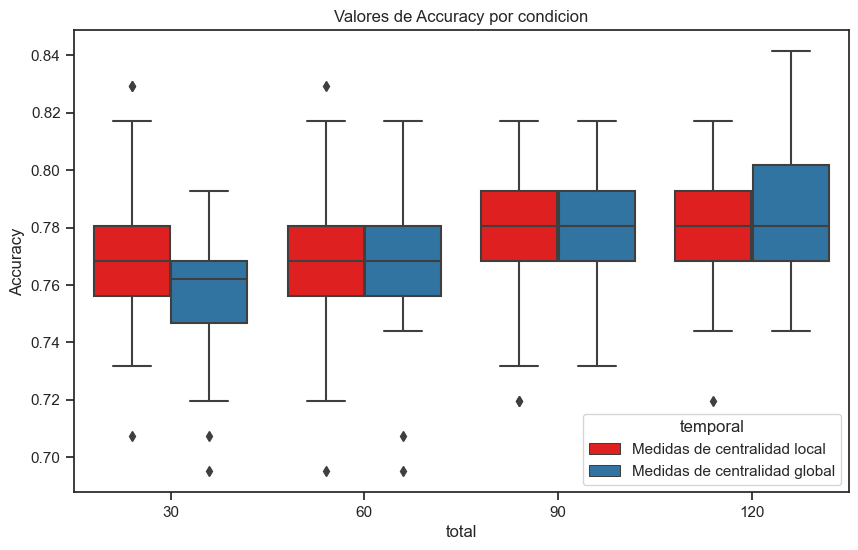
\includegraphics[width=0.8\textwidth]{figs/cap7/figura_38}
				\caption{Figura 10.7. Eficacia por rangos de tiempo y tipos de medidas (híbridas)}
			\end{figure}      
		\end{column}
		% create the column with the second image, that also
		% occupies half of the slide
		\begin{column}{.5\textwidth}
			\begin{figure}
				\centering
				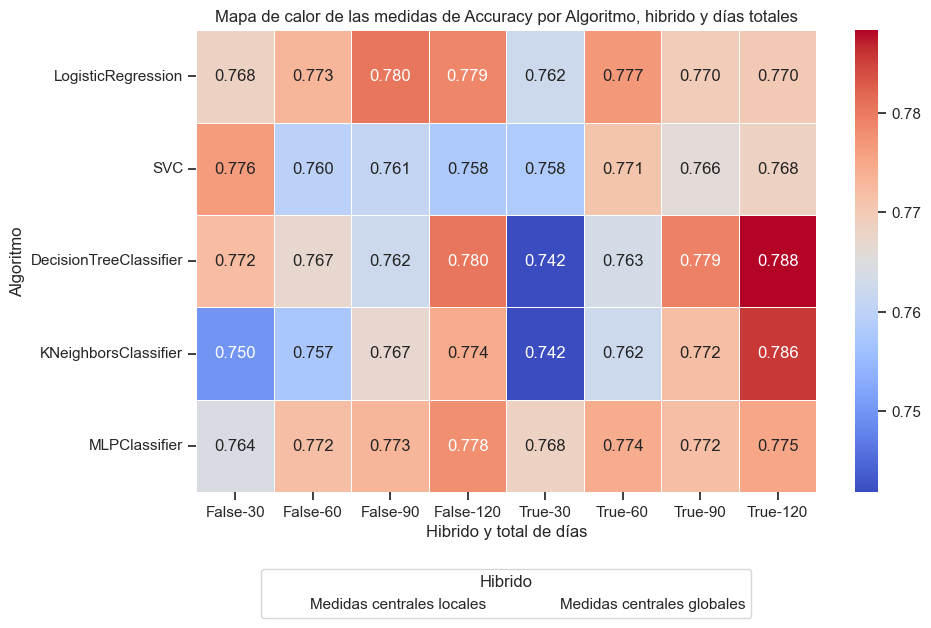
\includegraphics[width=0.8\textwidth]{figs/cap7/figura_90}
				\caption{Figura 7.76. Eficacia de los algoritmos por tipos de medidas (híbridas)}
			\end{figure}
		\end{column}
	\end{columns}
\end{frame}



%%========= Diapositiva con ítems resaltados con colores:
\begin{frame}
	\frametitle{Subobjetivo 2: Analizar la eficacia de las predicciones utilizando medidas centrales  locales vs globales (híbridas)}
	\begin{block}{Hipótesis de la Estructura Social Cognitivo }
Las medidas de centralidad \textcolor{blue}{globales} que evalúan la posición en la red de los nodos vecinos son ligeramente más eficaces para predecir el abandono de la asignatura.
	\end{block}
	
	\begin{columns}[c]
		% create the column with the first image, that occupies
		% half of the slide
		\begin{column}{.5\textwidth}
			\begin{figure}
				\centering
				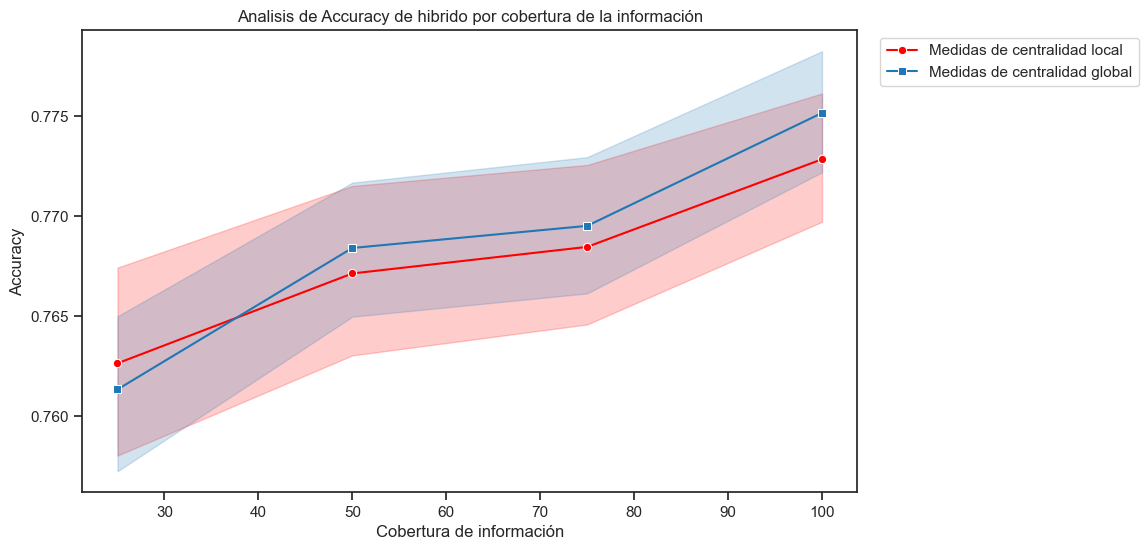
\includegraphics[width=1\textwidth]{figs/cap7/figura_43}
				\caption{Figura 10.9. Índice de amplitud de información}
			\end{figure}      
		\end{column}
		% create the column with the second image, that also
		% occupies half of the slide
		\begin{column}{.5\textwidth}
			\begin{figure}
				\centering
				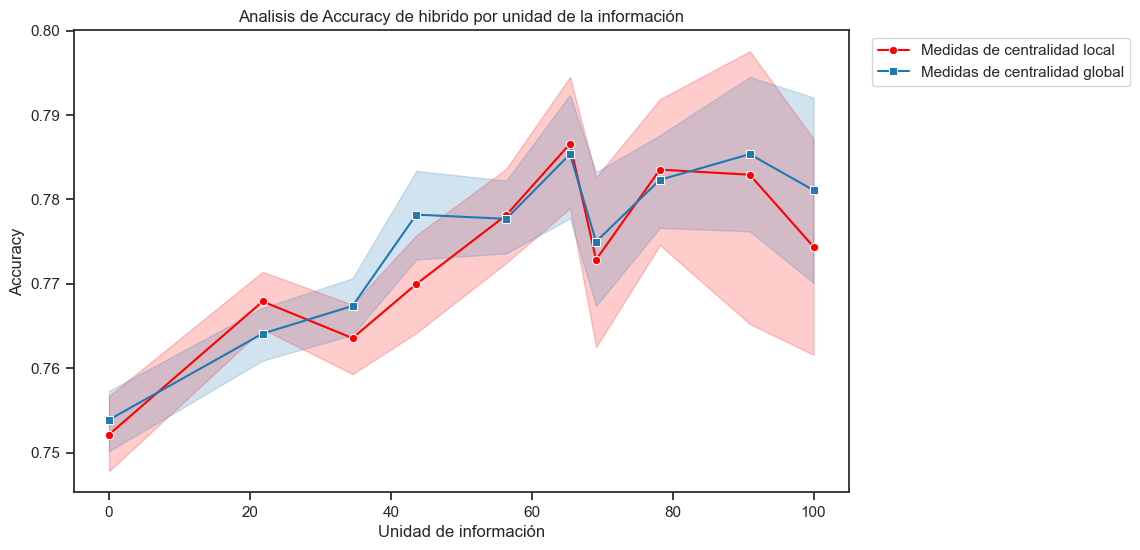
\includegraphics[width=1\textwidth]{figs/cap7/figura_44}
				\caption{Figura 10.10. Índice de unidad de información}
			\end{figure}
		\end{column}
	\end{columns}
	
\end{frame}

%========= Diapositiva con ítems resaltados con colores:
\begin{frame}
	\frametitle{Subobjetivo 2: Analizar la eficacia de las predicciones utilizando medidas centrales  locales vs globales (híbridas)}
\begin{block}{Hipótesis de la Estructura Social Cognitivo }
Las medidas de centralidad \textcolor{blue}{globales} tienden a ser más beneficiosas cuando se dispone de una mayor  \textcolor{red}{cantidad} de información.
\end{block}
	\begin{columns}[c]
		% create the column with the first image, that occupies
		% half of the slide
		\begin{column}{.5\textwidth}
			\begin{figure}
				\centering
				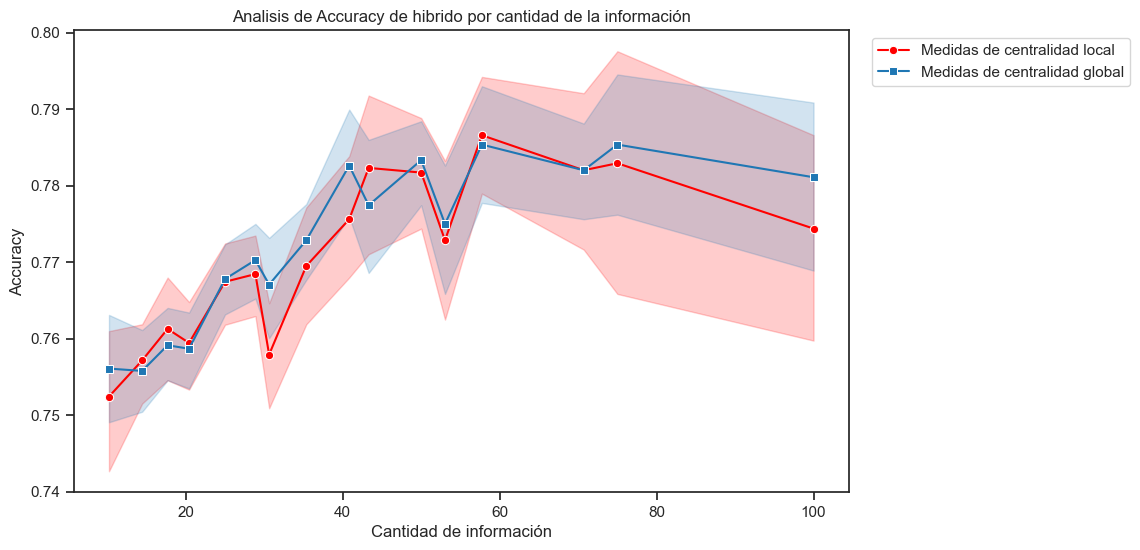
\includegraphics[width=0.9\textwidth]{figs/cap7/figura_45}
				\caption{Figura 10.11. Índice de cantidad de información}
			\end{figure}      
		\end{column}
		% create the column with the second image, that also
		% occupies half of the slide
		\begin{column}{.5\textwidth}
			\begin{figure}
				\centering
				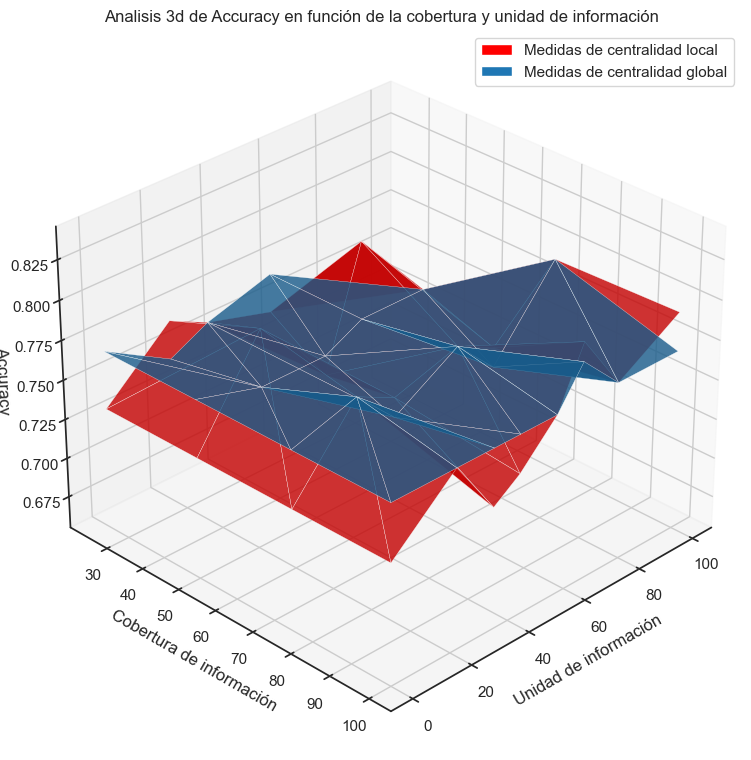
\includegraphics[width=0.6\textwidth]{figs/cap7/figura_46}
			\caption{Figura 10.12. Cobertura y unidad de información}
			\end{figure}
		\end{column}
	\end{columns}
\end{frame}






\subsection{Subobjetivo 3: Hipótesis del Balance Social Cognitivo}


%========= Diapositiva con ítems resaltados con colores:
\begin{frame}
	\frametitle{Subobjetivo 3: Analizar la eficacia de las predicciones utilizando medidas centrales y de sentimentos.}
	\begin{block}{Hipótesis del Balance Social Cognitivo}
		La precisión utilizando medidas de \textcolor{blue}{centralidad} y de \textcolor{red}{sentimiento} conjuntamente es similar o superior con la mayoría de algoritmos de aprendizaje y mejor en los rangos de tiempo intermedios (\textcolor{blue}{50-75\%}).
		
	\end{block}	
	\begin{columns}[c]
		% create the column with the first image, that occupies
		% half of the slide
		\begin{column}{.5\textwidth}
			\begin{figure}
				\centering
				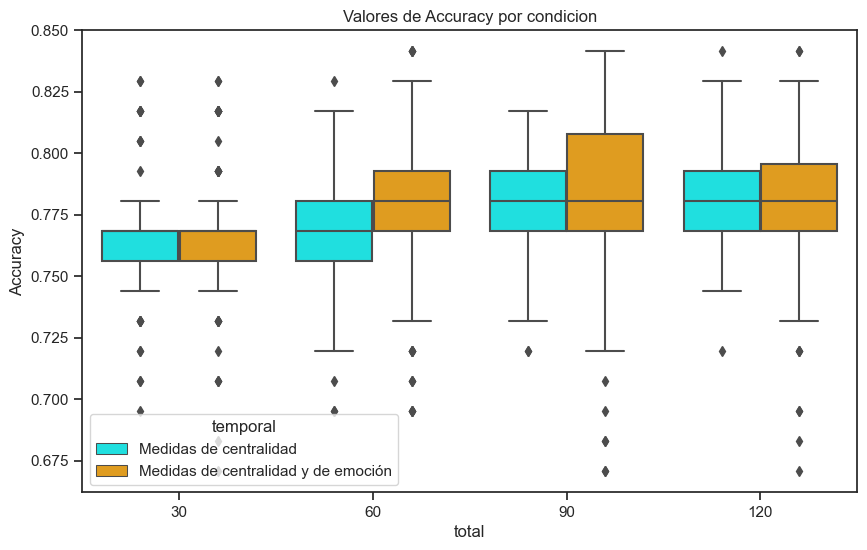
\includegraphics[width=0.8\textwidth]{figs/cap7/figura_48}
				\caption{Figura 10.13. Eficacia por rangos de tiempo y tipos de medidas (sentimiento)}
			\end{figure}      
		\end{column}
		% create the column with the second image, that also
		% occupies half of the slide
		\begin{column}{.5\textwidth}
			\begin{figure}
				\centering
				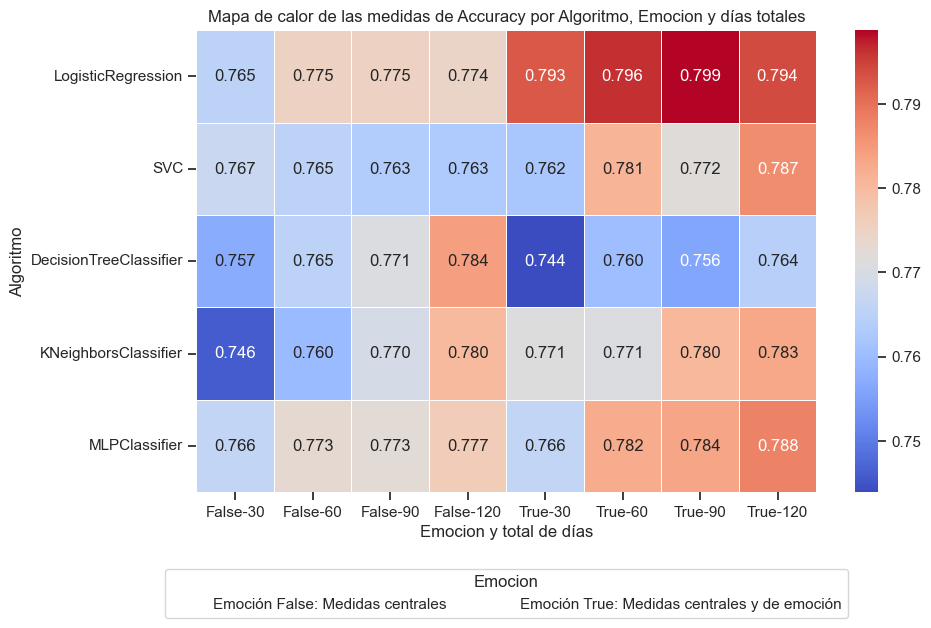
\includegraphics[width=0.8\textwidth]{figs/cap7/figura_111}
				\caption{Figura 7.90. Eficacia de los algoritmos por tipos de medidas (sentimiento)}
			\end{figure}
		\end{column}
	\end{columns}	
\end{frame}

%%========= Diapositiva con ítems resaltados con colores:
\begin{frame}
	\frametitle{Subobjetivo 3: Analizar la eficacia de las predicciones utilizando medidas centrales y de sentimentos.}
	\begin{block}{Hipótesis del Balance Social Cognitivo}
El uso conjunto de medidas \textcolor{red}{emocionales} y de \textcolor{blue}{centralidad} mejora la capacidad predictiva del modelo.

	\end{block}
			\begin{columns}[c]
		% create the column with the first image, that occupies
		% half of the slide
		\begin{column}{.5\textwidth}
			\begin{figure}
				\centering
				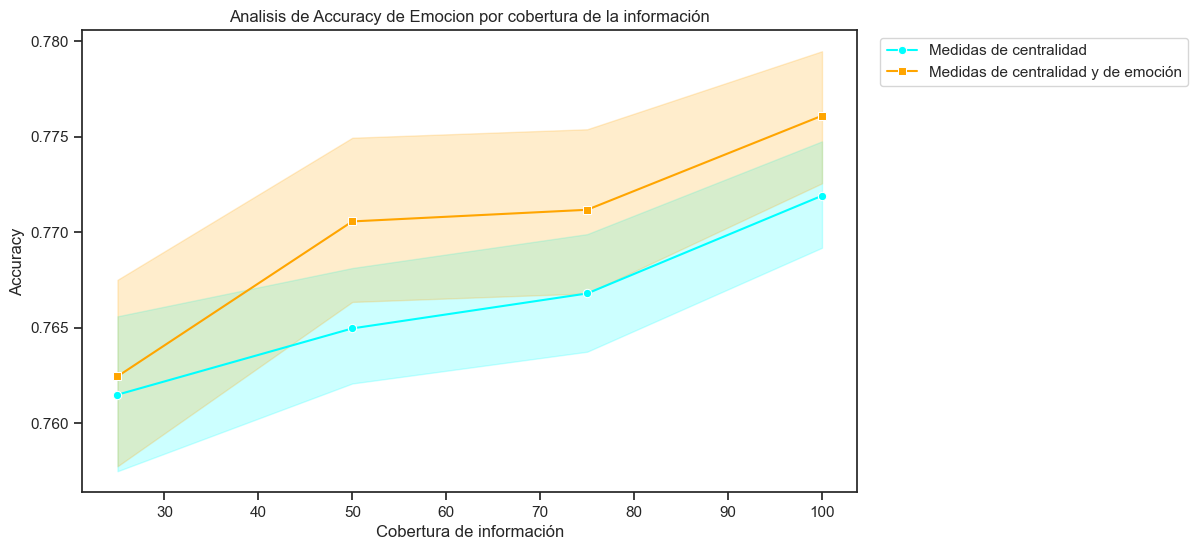
\includegraphics[width=1\textwidth]{figs/cap7/figura_53}
\caption{Figura 10.15. Índice de amplitud de información}
			\end{figure}      
		\end{column}
		% create the column with the second image, that also
		% occupies half of the slide
		\begin{column}{.5\textwidth}
			\begin{figure}
				\centering
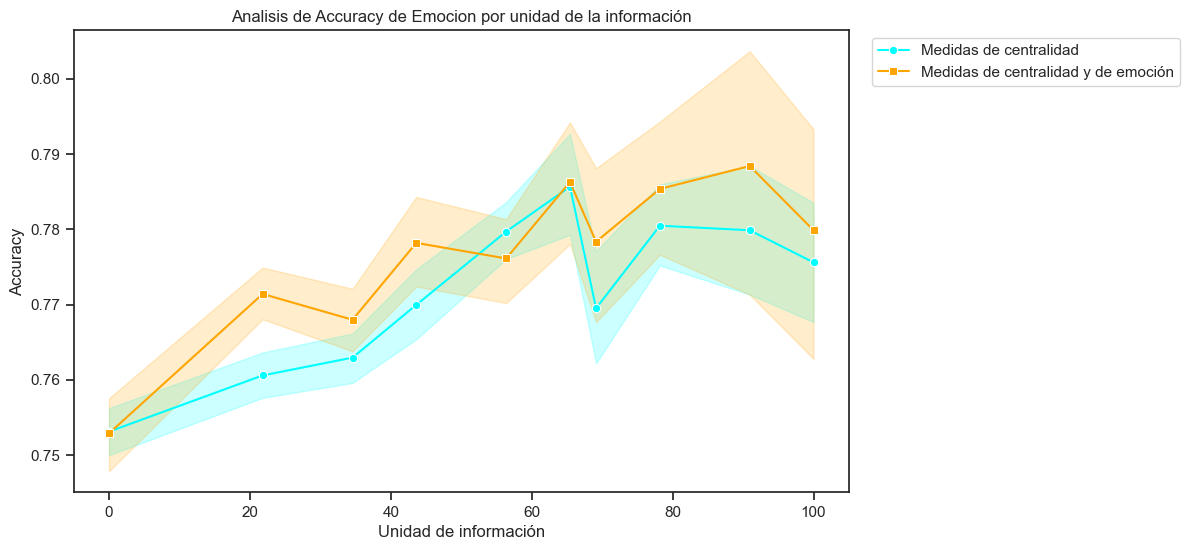
\includegraphics[width=1\textwidth]{figs/cap7/figura_54}
\caption{Figura 10.16. Índice de unidad de información}
			\end{figure}
		\end{column}
	\end{columns}
	
\end{frame}



%========= Diapositiva con ítems resaltados con colores:
\begin{frame}
	\frametitle{Subobjetivo 3: Analizar la eficacia de las predicciones utilizando medidas centrales y de sentimentos.}
\begin{block}{Hipótesis del Balance Social Cognitivo}
Las medidas de \textcolor{blue}{centralidad} y de \textcolor{red}{sentimiento} conjuntamente pueden ser mejores para la predicción cuanto mayor \textcolor{blue}{cantidad} de información.

\end{block}	
	\begin{columns}[c]
		% create the column with the first image, that occupies
		% half of the slide
		\begin{column}{.5\textwidth}
			\begin{figure}
				\centering
				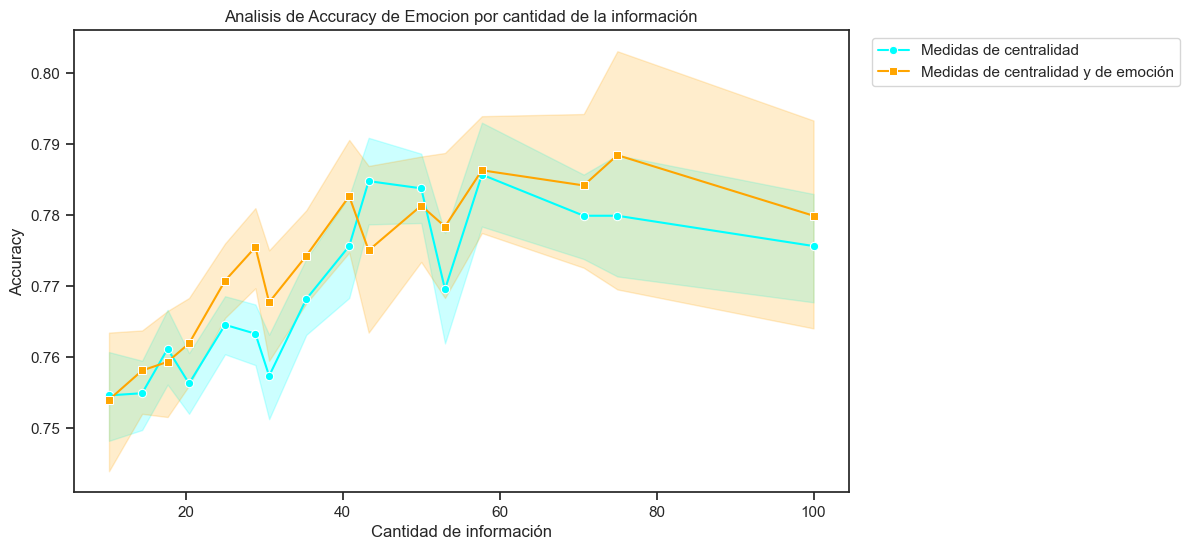
\includegraphics[width=1\textwidth]{figs/cap7/figura_55}
				\caption{Figura 10.17. Índice de cantidad de información}
			\end{figure}      
		\end{column}
		% create the column with the second image, that also
		% occupies half of the slide
		\begin{column}{.5\textwidth}
			\begin{figure}
				\centering
				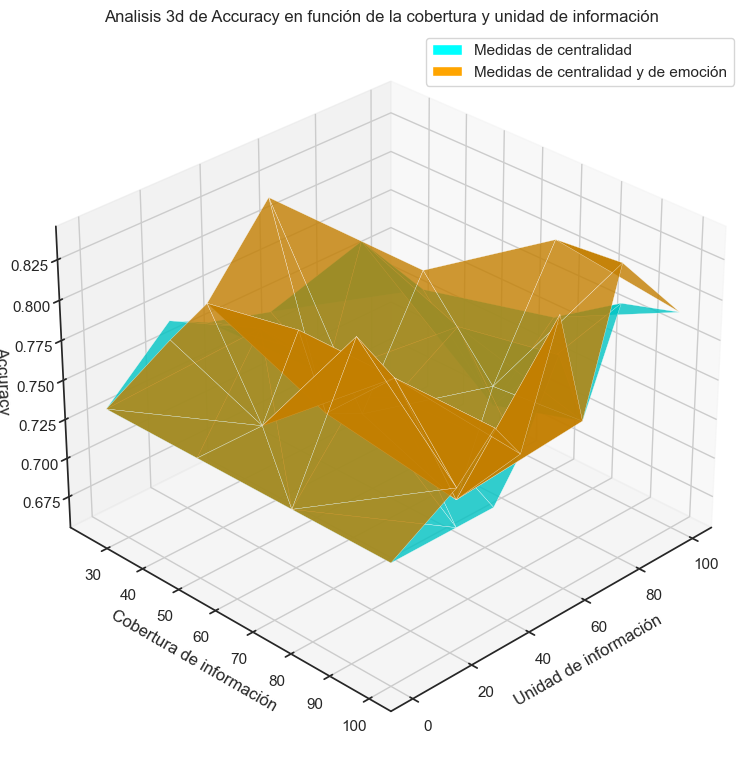
\includegraphics[width=0.60\textwidth]{figs/cap7/figura_56}
			\caption{Figura 10.18. Cobertura y unidad de información.}
			\end{figure}
		\end{column}
	\end{columns}
	
\end{frame}






\section{Conclusiones}
%\begin{frame}
%	\frametitle{Resultados clave}
%  \begin{itemize}
%	\item A medida que aumenta el porcentaje de cobertura temporal, la eficacia de todos los tipos de subdivisión en bloques también incrementa.
%	
%	\item Existe un equilibrio entre la cantidad (amplitud x unidad) de información analizada y la capacidad predictiva del modelo, ya que el punto máximo de eficacia en la predicción no se encuentra en el máximo nivel de cobertura temporal.
%	
%	\item La subdivisión del análisis de la red social en bloques temporales encadenados muestra una eficacia superior en comparación con la subdivisión en bloques secuenciales.
%	
%	\item Las medidas de centralidad globales que evalúan la posición en la red de los nodos vecinos pueden ser más eficaces para capturar la estructura de la red del estudiante y predecir su abandono de la asignatura.
%	
%	\item La integración de medidas emocionales con las medidas de centralidad mejora la capacidad predictiva del modelo.
%
%\end{itemize}
%\end{frame}



\begin{frame}
	\frametitle{Limitaciones y futuras investigaciones}
	
	\begin{itemize}
		\item Tamaño limitado y sesgado de los datos analizados.
		\item Uso de medidas de cohesión de la red y algoritmos de detección de comunidades diferentes.
		\item Integración de medidas de centralidad y análisis de sentimiento para comprender la relación entre emociones y posición de los nodos.
		\item Utilización de técnicas de balanceo de datos, como SMOTE, para abordar el desbalance de los datos.
		\item Evaluación de la importancia relativa de las características mediante la técnica SHAP.
		\item Implementación de técnicas de ensamblaje, como Bagging o RandomForest.
	\end{itemize}
\end{frame}



\begin{frame}
	\frametitle{Aplicación de los resultados}
	
	\begin{enumerate}
		\item Identificación temprana de estudiantes en riesgo: El análisis de la interacción en los foros de las asignaturas, considerando medidas de centralidad y evaluaciones emocionales, puede ayudar a identificar a los estudiantes que están en riesgo de abandonar la asignatura o que están experimentando dificultades académicas.
		
		\item Diseño de estrategias de enseñanza personalizadas: La comprensión de los patrones de comportamiento y las preferencias de los estudiantes en los foros de la asignatura puede guiar el diseño de estrategias de enseñanza personalizadas.
		
		\item Mejora de la experiencia del estudiante en entornos de aprendizaje en línea: El análisis de medidas de centralidad y evaluaciones emocionales en los foros de las asignaturas puede proporcionar información valiosa para mejorar la experiencia del estudiante en entornos virtuales.
		
		\item Desarrollo de sistemas de recomendación personalizados: La combinación de medidas de centralidad y emocionales puede ser utilizada para desarrollar sistemas de recomendación personalizados.
	\end{enumerate}
\end{frame}


\begin{frame}[plain]
\large{\titlepage}
\note[item]{Y hasta aquí mi exposición.}
\note[item]{Quedo a disposición del tribunal...}
\end{frame}



%%%
% CONTENIDO. BIBLIOGRAFÍA.
%%%%
%\nocite{*} %incluye TODOS los documentos de la base de datos bibliográfica sean o no citados en el texto
\bibliography{bibliografia/bibliografia} % Archivo que contiene la bibliografía
%\bibliographystyle{apacite}
\bibliographystyle{IEEEtranN}
%\bibliographystyle{amsplain}

\end{document}
